\section{Radiant System Models }\label{radiant-system-models}

\subsection{Low Temperature Radiant System Model}\label{low-temperature-radiant-system-model}

The input objects ZoneHVAC:LowTemperatureRadiant:ConstantFlow, \\ ZoneHVAC:LowTemperatureRadiant:VariableFlow, and \\
ZoneHVAC:LowTemperatureRadiant:Electric provide models for low temperature radiant heating and cooling systems that appear, on the surface, to be relatively simple systems.~ The system circulates hot or cold fluid through tubes embedded in a wall, ceiling, or floor or runs current through electric resistance wires embedded in a surface or a panel.~ Energy is thus either added to or removed from the space, and zone occupants are conditioned by both radiation exchange with the system and convection from the surrounding air that is also affected by the system.~ Unless specifically required for indoor air quality considerations, fans, ductwork, dampers, etc. are not needed.

Despite the relative simplicity of the low temperature radiant systems, the integration of such a system within an energy analysis program requires one to overcome several challenges.~ First, for systems with significant thermal mass, the conduction transfer function method for modeling transient conduction must be extended to include embedded heat sources or sinks.~ Second, one must integrate this formulation within an energy analysis program like EnergyPlus.~ Finally, one must overcome the fact that the radiant system is both a zone heat balance element and a conditioning system.~ Each of these issues will be addressed in the next several subsections.

\subsubsection{One Dimensional Heat Transfer Through Multilayered Slabs}\label{one-dimensional-heat-transfer-through-multilayered-slabs}

One of the most important forms of heat transfer in energy analysis is heat conduction through building elements such as walls, floors, and roofs.~ While some thermally lightweight structures can be approximated by steady state heat conduction, a method that applies to all structures must account for the presence of thermal mass within the building elements.~ Transient one dimensional heat conduction through a homogeneous layer with constant thermal properties such as the one shown in Figure~\ref{fig:single-layered-building-element} is governed by the following equation:

\begin{equation}
\frac{{{\partial ^2}T}}{{\partial {x^2}}} = \frac{1}{\alpha }\frac{{\partial T}}{{\partial t}}
\end{equation}

where: T is the temperature as a function of position and time,

x is the position,

t is the time,

\(\alpha = \frac{k}{{\rho {c_p}}}\) ~is the thermal diffusivity of the layer material,

k is its thermal conductivity,

r is its density, and

cp~is its specific heat.

This equation is typically coupled with Fourier's law of conduction that relates the heat flux at any position and time to temperature as follows:

\begin{equation}
q''\left( {x,t} \right) =  - k\frac{{\partial T\left( {x,t} \right)}}{{\partial x}}
\end{equation}

\begin{figure}[hbtp] % fig 266
\centering
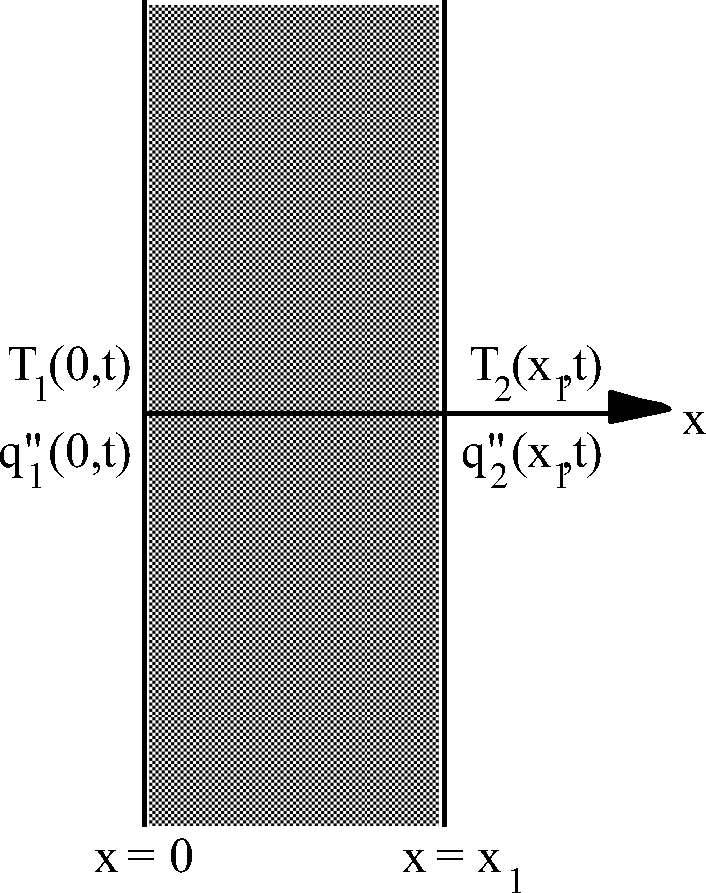
\includegraphics[width=0.9\textwidth, height=0.9\textheight, keepaspectratio=true]{media/image5973.png}
\caption{Single Layered Building Element \protect \label{fig:single-layered-building-element}}
\end{figure}

While analytical solutions exist for the single homogeneous layer shown in Figure~\ref{fig:single-layered-building-element}, the solution becomes extremely tedious for the multiple layered slab shown in Figure~\ref{fig:multilayered-building-element}.

\begin{figure}[hbtp] % fig 267
\centering
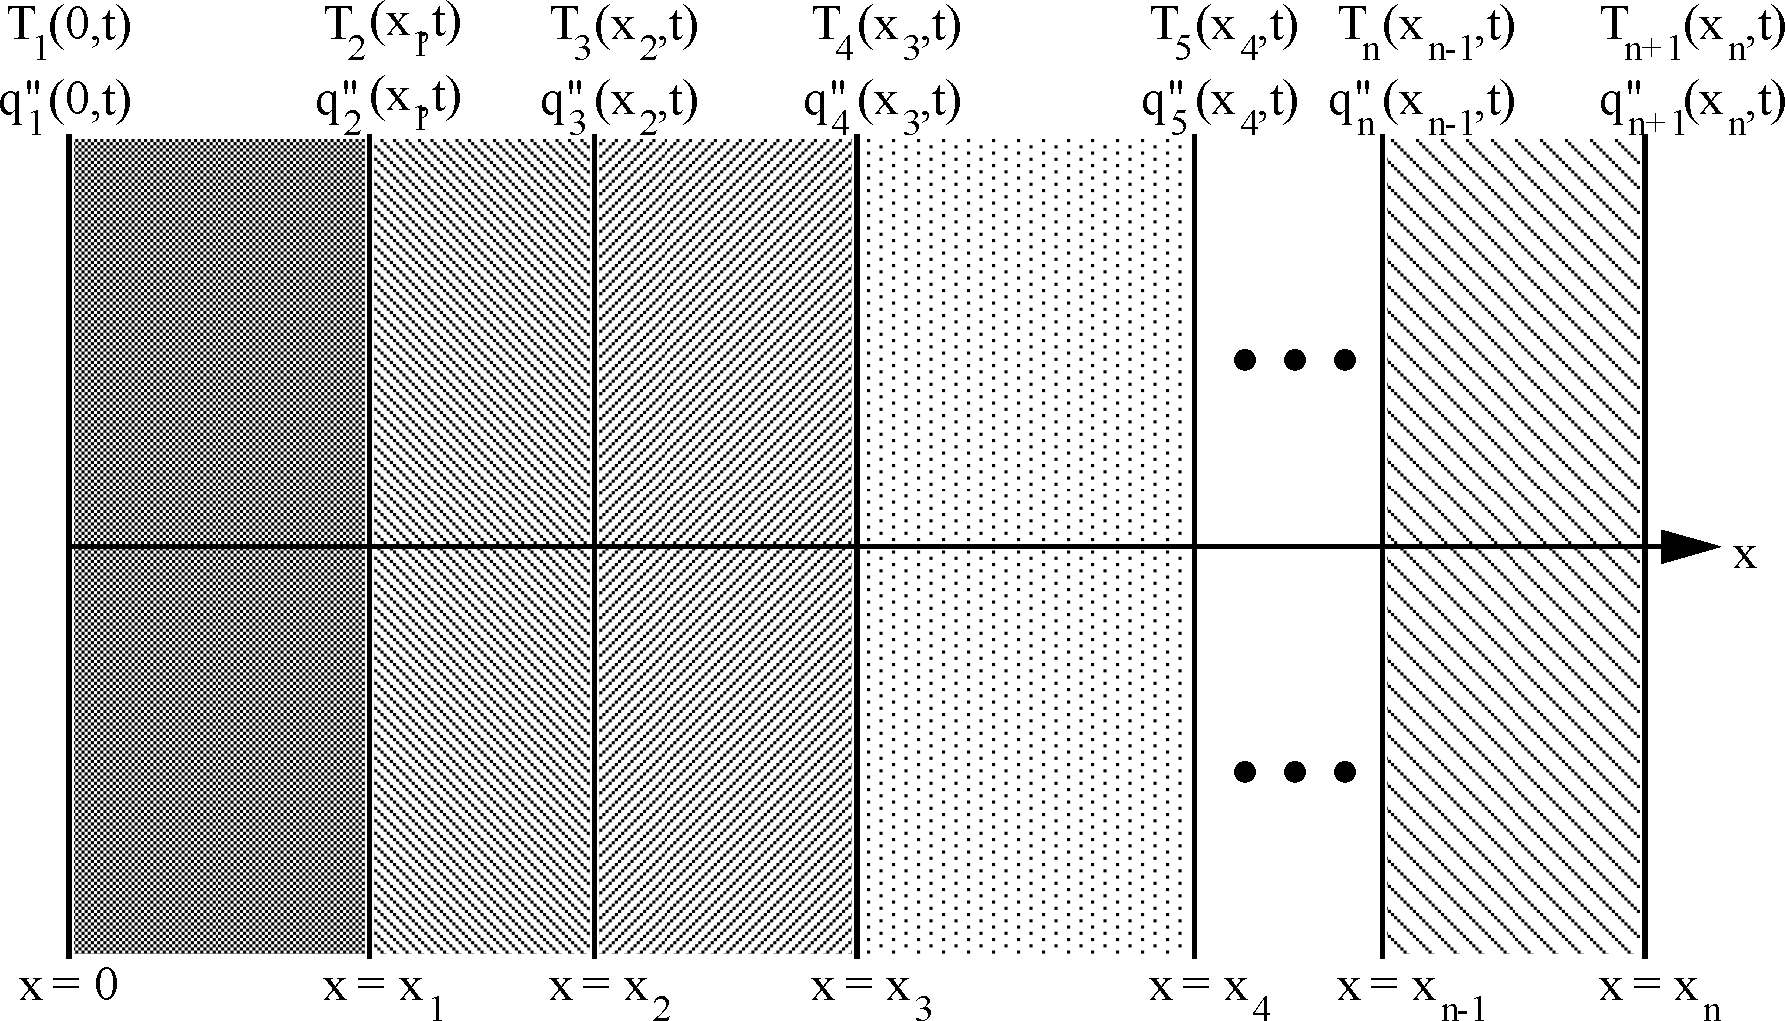
\includegraphics[width=0.9\textwidth, height=0.9\textheight, keepaspectratio=true]{media/image5974.png}
\caption{Multilayered Building Element \protect \label{fig:multilayered-building-element}}
\end{figure}

\subsubsection{Time Series Solutions:~ Conduction Transfer Functions}\label{time-series-solutions-conduction-transfer-functions}

Equations and can be solved numerically in a variety of ways.~ As mentioned in the previous section, other models have used control theory and numerical methods such as finite difference and finite element.~ However, each of these methods have drawbacks which render them inappropriate for use within an energy analysis program which requires both accuracy and efficiency from the simulation.

Another possible modeling method is a time series solution.~ Several of the detailed energy analysis programs such as EnergyPlus use a time series solution to transient heat conduction.~ The most basic time series solution is the response factor equation which relates the flux at one surface of an element to an infinite series of temperature histories at both sides as shown by:

\begin{equation}
{q''_{i,t}} = \sum\limits_{m = 1}^\infty  {{X_m}{T_{i,t - m + 1}}}  - \sum\limits_{m = 1}^\infty  {{Y_m}{T_{o,t - m + 1}}}
\end{equation}

where q'' is heat flux, T is temperature, i signifies the inside of the building element, o signifies the outside of the building element, and t represents the current time step.

While in most cases the terms in the series decay fairly rapidly, the infinite number of terms needed for an exact response factor solution makes it less than desirable.~ Fortunately, the similarity of higher order terms can be used to replace them with flux history terms.~ The new solution contains elements that are called conduction transfer functions (CTFs).~ The basic form of a conduction transfer function solution is shown by the following equation:

\begin{equation}
{q''_{i,t}} = \sum\limits_{m = 1}^M {{X_m}{T_{i,t - m + 1}}}  - \sum\limits_{m = 1}^M {{Y_m}{T_{o,t - m + 1}}}  + \sum\limits_{m = 1}^k {{F_m}{{q''}_{i,t - m}}}
\end{equation}

where k is the order of the conduction transfer functions, M is a finite number defined by the order of the conduction transfer functions, and X, Y, and F are the conduction transfer functions.~ This equation states that the heat flux at the interior surface of any generic building element for which the assumption of one dimensional conduction heat transfer is valid is linearly related to the current and some of the previous temperatures at both the interior and exterior surface as well as some of the previous flux values at the interior surface.~ A similar equation holds for the heat flux at the exterior surface.

The final CTF solution form reveals why it is so elegant and powerful.~ With a single, relatively simple equation, the conduction heat transfer through an element can be calculated.~ The coefficients (CTFs) in the equation are constants that only need to be determined once.~ The only storage of data required is the CTFs themselves and a limited number of temperature and flux terms.~ The formulation is valid for any surface type and does not require the calculation or storage of element interior temperatures.

As the next several sections will detail, there are two main methods for calculating conduction transfer functions:~ the Laplace Transform method and the State Space method.~ Both methods are well suited for the main focus of this research, the extension of conduction transfer functions to include heat sources or sinks.

\subsubsection{Laplace Transform Formulation}\label{laplace-transform-formulation}

The traditional method for calculating conduction transfer functions is described in detail by Hittle (1981).~ Beginning with the transient one dimensional heat conduction equation \{Equation \} and Fourier's law of conduction \{Equation \}, the Laplace transform method is used to convert the governing equations into the s-domain for a single layer such as the one shown in Figure~\ref{fig:single-layered-building-element}.

\begin{equation}
\frac{{{d^2}T\left( {x,s} \right)}}{{d{x^2}}} = \frac{s}{\alpha }T\left( {x,s} \right)
\end{equation}

\begin{equation}
q''\left( {x,s} \right) =  - k\frac{{dT\left( {x,s} \right)}}{{dx}}
\end{equation}

The transformed equations are solved and then put in matrix form as shown below:

\begin{equation}
\left[ 
    {\begin{array}{*{20}{c}}
      {{T_1}\left( s \right)} \\ {{q_1}\left( s \right)}
    \end{array}}
  \right] = \left[ 
    {\begin{array}{*{20}{c}}
      {{A_1}\left( s \right)}&{{B_1}\left( s \right)} \\
      {{C_1}\left( s \right)}&{{D_1}\left( s \right)}
    \end{array}}
  \right] \left[ 
    {\begin{array}{*{20}{c}}
      {{T_2}\left( s \right)} \\
      {{q_2}\left( s \right)}
    \end{array}}
  \right]
\end{equation}

where: T1(s), T2(s), q1(s), and q2(s) are the temperature and flux terms in the Laplace domain,

\({A_1}\left( s \right) = \cosh \left( {{\ell_1}\sqrt {{s \mathord{\left/ {\vphantom {s {{\alpha_1}}}} \right. } {{\alpha_1}}}} } \right)\) ,

\({B_1}\left( s \right) = \left( {{1 \mathord{\left/ {\vphantom {1 {{k_1}\sqrt {{s \mathord{\left/ {\vphantom {s {{\alpha_1}}}} \right. } {{\alpha_1}}}} }}} \right. } {{k_1}\sqrt {{s \mathord{\left/ {\vphantom {s {{\alpha_1}}}} \right. } {{\alpha_1}}}} }}} \right)\sinh \left( {{\ell_1}\sqrt {{s \mathord{\left/ {\vphantom {s {{\alpha_1}}}} \right. } {{\alpha_1}}}} } \right)\) ,

\({C_1}\left( s \right) = {k_1}\sqrt {{s \mathord{\left/ {\vphantom {s {{\alpha_1}}}} \right. } {{\alpha_1}}}} \sinh \left( {{\ell_1}\sqrt {{s \mathord{\left/ {\vphantom {s {{\alpha_1}}}} \right. } {{\alpha_1}}}} } \right)\) ,

\({D_1}\left( s \right) = \cosh \left( {{\ell_1}\sqrt {{s \mathord{\left/ {\vphantom {s {{\alpha_1}}}} \right. } {{\alpha_1}}}} } \right)\) ,

k1~is the thermal conductivity of the layer,

a1~is the thermal diffusivity of the layer, and

\({\ell_1}\) ~is the thickness of the layer.

The 2 x 2 matrix consisting of A1(s), B1(s), C1(s), and D1(s) is called the transmission matrix and contains all of the thermophysical properties of the layer necessary to calculate transient conduction heat transfer through it.~ It can easily be shown that a second layer could be characterized in a similar way as:

\begin{equation}
\left[ {\begin{array}{*{20}{c}}{{T_2}\left( s \right)}\\ {{q_2}\left( s \right)}\end{array}} \right] = \left[ {\begin{array}{*{20}{c}}{{A_2}\left( s \right)}&{{B_2}\left( s \right)}\\ {{C_2}\left( s \right)}&{{D_2}\left( s \right)}\end{array}} \right]\left[ {\begin{array}{*{20}{c}}{{T_3}\left( s \right)}\\ {{q_3}\left( s \right)}\end{array}} \right]
\end{equation}

where A2(s), B2(s), C2(s), and D2(s) are calculated using the properties of the second layer.~ This can be substituted into Equation to provide insight how the extension to multilayered slabs is achieved.

\begin{equation}
\left[ {\begin{array}{*{20}{c}}{{T_1}\left( s \right)}\\ {{q_1}\left( s \right)}\end{array}} \right] = \left[ {\begin{array}{*{20}{c}}{{A_1}\left( s \right)}&{{B_1}\left( s \right)}\\ {{C_1}\left( s \right)}&{{D_1}\left( s \right)}\end{array}} \right]\left[ {\begin{array}{*{20}{c}}{{A_2}\left( s \right)}&{{B_2}\left( s \right)}\\ {{C_2}\left( s \right)}&{{D_2}\left( s \right)}\end{array}} \right]\left[ {\begin{array}{*{20}{c}}{{T_3}\left( s \right)}\\ {{q_3}\left( s \right)}\end{array}} \right]
\end{equation}

Thus, for a multilayered element as shown in Figure~\ref{fig:multilayered-building-element}, each separate layer has a transmission matrix of Ai(s), Bi(s), Ci(s), and Di(s) associated with it.~ The form of the matrix equation for the multilayered element is the same as the equation for a single layer:

\begin{equation}
\left[ {\begin{array}{*{20}{c}}{{T_1}\left( s \right)}\\ {{q_1}\left( s \right)}\end{array}} \right] = \left[ {\begin{array}{*{20}{c}}{A\left( s \right)}&{B\left( s \right)}\\ {C\left( s \right)}&{D\left( s \right)}\end{array}} \right]\left[ {\begin{array}{*{20}{c}}{{T_{n + 1}}\left( s \right)}\\ {{q_{n + 1}}\left( s \right)}\end{array}} \right]
\end{equation}

but the transmission matrix is replaced by:

\begin{equation}
\left[ {\begin{array}{*{20}{c}}{A\left( s \right)}&{B\left( s \right)}\\ {C\left( s \right)}&{D\left( s \right)}\end{array}} \right] = \left[ {\begin{array}{*{20}{c}}{{A_1}\left( s \right)}&{{B_1}\left( s \right)}\\ {{C_1}\left( s \right)}&{{D_1}\left( s \right)}\end{array}} \right]\left[ {\begin{array}{*{20}{c}}{{A_2}\left( s \right)}&{{B_2}\left( s \right)}\\ {{C_2}\left( s \right)}&{{D_2}\left( s \right)}\end{array}} \right] \cdots \left[ {\begin{array}{*{20}{c}}{{A_n}\left( s \right)}&{{B_n}\left( s \right)}\\ {{C_n}\left( s \right)}&{{D_n}\left( s \right)}\end{array}} \right]
\end{equation}

Equation is typically rearranged as follows:

\begin{equation}
\left[ {\begin{array}{*{20}{c}}{{q_1}\left( s \right)}\\ {{q_{n + 1}}\left( s \right)}\end{array}} \right] = \left[ {\begin{array}{*{20}{c}}{\frac{{D\left( s \right)}}{{B\left( s \right)}}}&{\frac{{ - 1}}{{B\left( s \right)}}}\\ {\frac{1}{{B\left( s \right)}}}&{\frac{{ - A\left( s \right)}}{{B\left( s \right)}}}\end{array}} \right]\left[ {\begin{array}{*{20}{c}}{{T_1}\left( s \right)}\\ {{T_{n + 1}}\left( s \right)}\end{array}} \right]
\end{equation}

which relates the flux at either surface of the element to the temperature histories at both surfaces.~ When the temperature histories are formulated as triangular pulses made up of simple ramp functions, the roots of this equation can be found and result in response factors.~ The response factors can be simplified as described above through the introduction of flux history terms to form conduction transfer functions.~ A simplified method of finding the roots of the Laplace domain equations is described by Hittle and Bishop (1983) and is used by the current version of BLAST.

\subsubsection{State Space Formulation}\label{state-space-formulation}

Recently, another method of finding conduction transfer functions starting from a state space representation has begun receiving increased attention (Ceylan and Myers 1980; Seem 1987; Ouyang and Haghighat 1991).~ The basic state space system is defined by the following linear matrix equations:

\begin{equation}
\frac{{d\left[ x \right]}}{{dt}} = \left[ A \right]\left[ x \right] + \left[ B \right]\left[ u \right]
\end{equation}

\begin{equation}
\left[ y \right] = \left[ C \right]\left[ x \right] + \left[ D \right]\left[ u \right]
\end{equation}

where x is a vector of state variables, u is a vector of inputs, y is the output vector, t is time, and A, B, C, and D are coefficient matrices.~ Through the use of matrix algebra, the vector of state variables (x) can be eliminated from the system of equations, and the output vector (y) can be related directly to the input vector (u) and time histories of the input and output vectors.

This formulation can be used to solve the transient heat conduction equation by enforcing a finite difference grid over the various layers in the building element being analyzed.~ In this case, the state variables are the nodal temperatures, the environmental temperatures (interior and exterior) are the inputs, and the resulting heat fluxes at both surfaces are the outputs.~ Thus, the state space representation with finite difference variables would take the following form:

\begin{equation}
\frac{{d\left[ {\begin{array}{*{20}{c}}{{T_1}}\\ \vdots \\ {{T_n}}\end{array}} \right]}}{{dt}} = \left[ A \right]\left[ {\begin{array}{*{20}{c}}{{T_1}}\\ \vdots \\ {{T_n}}\end{array}} \right] + \left[ B \right]\left[ {\begin{array}{*{20}{c}}{{T_i}}\\ {{T_o}}\end{array}} \right]
\end{equation}

\begin{equation}
\left[ {\begin{array}{*{20}{c}}{{{q''}_i}}\\ {{{q''}_o}}\end{array}} \right] = \left[ C \right]\left[ {\begin{array}{*{20}{c}}{{T_1}}\\ \vdots \\ {{T_n}}\end{array}} \right] + \left[ D \right]\left[ {\begin{array}{*{20}{c}}{{T_i}}\\ {{T_o}}\end{array}} \right]
\end{equation}

where T1, T2, \ldots{}, Tn-1, Tn~are the finite difference nodal temperatures, n is the number of nodes, Ti~and To~are the interior and exterior environmental temperatures, and \({q''_i}\) ~and \({q''_o}\) ~are the heat fluxes (desired output).

Seem (1987) shows that for a simple one layer slab with two interior nodes as in Figure~\ref{fig:two-node-state-space-example} and convection at both sides the resulting finite difference equations are given by:

\begin{equation}
C\frac{{d{T_1}}}{{dt}} = hA\left( {{T_o} - {T_1}} \right) + \frac{{{T_2} - {T_1}}}{R}
\end{equation}

\begin{equation}
C\frac{{d{T_2}}}{{dt}} = hA\left( {{T_i} - {T_2}} \right) + \frac{{{T_1} - {T_2}}}{R}
\end{equation}

\begin{equation}
{q''_i} = h\left( {{T_i} - {T_2}} \right)
\end{equation}

\begin{equation}
{q''_o} = h\left( {{T_1} - {T_o}} \right)
\end{equation}

where:~~~~~~~~ \(R = \frac{\ell }{{kA}}\) ~ , thermal resistance

\(C = \frac{{\rho {c_p}\ell A}}{2}\) ~, thermal capacitance

\({T_o}\) = outside temperature

\({T_i}\) = inside temperature

\({T_1}\) = temperature of node 1

\({T_2}\) = temperature of node 2

and

A is the area of the surface exposed to the environmental temperatures.

In matrix format:

\begin{equation}
\left[ {\begin{array}{*{20}{c}}{\frac{{d{T_1}}}{{dt}}}\\ {\frac{{d{T_2}}}{{dt}}}\end{array}} \right] = \left[ {\begin{array}{*{20}{c}}{\frac{{ - 1}}{{RC}} - \frac{{hA}}{C}}&{\frac{1}{{RC}}}\\ {\frac{1}{{RC}}}&{\frac{{ - 1}}{{RC}} - \frac{{hA}}{C}}\end{array}} \right]\left[ {\begin{array}{*{20}{c}}{{T_1}}\\ {{T_2}}\end{array}} \right] + \left[ {\begin{array}{*{20}{c}}{\frac{{hA}}{C}}&0\\0&{\frac{{hA}}{C}}\end{array}} \right]\left[ {\begin{array}{*{20}{c}}{{T_o}}\\ {{T_i}}\end{array}} \right]
\end{equation}

\begin{equation}
\left[ {\begin{array}{*{20}{c}}{{{q''}_i}}\\ {{{q''}_o}}\end{array}} \right] = \left[ {\begin{array}{*{20}{c}}0&{ - h}\\h&0\end{array}} \right]\left[ {\begin{array}{*{20}{c}}{{T_1}}\\ {{T_2}}\end{array}} \right] + \left[ {\begin{array}{*{20}{c}}0&h\\ { - h}&0\end{array}} \right]\left[ {\begin{array}{*{20}{c}}{{T_o}}\\ {{T_i}}\end{array}} \right]
\end{equation}

\begin{figure}[hbtp] % fig 268
\centering
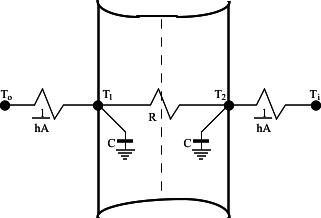
\includegraphics[width=0.9\textwidth, height=0.9\textheight, keepaspectratio=true]{media/image6008.svg.png}
\caption{Two Node State Space Example \protect \label{fig:two-node-state-space-example}}
\end{figure}

The important aspect of the state space technique is that through the use of relatively simple matrix algebra the state space variables (nodal temperatures) can be eliminated to arrive at a matrix equation that gives the outputs (heat fluxes) as a function of the inputs (environmental temperatures) only.~ This eliminates the need to solve for roots in the Laplace domain.~ In addition, the resulting matrix form has more physical meaning than complex functions required by the Laplace transform method.~ The current version of EnergyPlus uses the state space method for computing CTFs.

The accuracy of the state space method of calculating CTFs has been addressed in the literature.~ Ceylan and Myers (1980) compared the response predicted by the state space method to various other solution techniques including an analytical solution.~ Their results showed that for an adequate number of nodes the state space method computed a heat flux at the surface of a simple one layer slab within 1\% of the analytical solution.~ Ouyang and Haghighat (1991) made a direct comparison between the Laplace and state space methods.~ For a wall composed of insulation between two layers of concrete, they found almost no difference in the response factors calculated by each method.

\subsubsection{Extension of Time Series Solutions to Include Heat Sources and Obtain Internal Temperatures}\label{extension-of-time-series-solutions-to-include-heat-sources-and-obtain-internal-temperatures}

\subsubsection{Laplace Transform Formulation}\label{laplace-transform-formulation-1}

Degiovanni (1988) proposed two methodologies for including sources or sinks in the Laplace Transform Formulation.~ The first method shows how a source that varies as a function of time and location can be incorporated.~ The resulting equations involve some fairly complicated terms including spatial derivatives.

The second method that will be analyzed in more detail involves the addition of a source or sink at the interface between two layers.~ The derivation of the necessary equations is begun by analyzing the simple two layer element shown in Figure 269.

\begin{figure}[htbp]
\centering
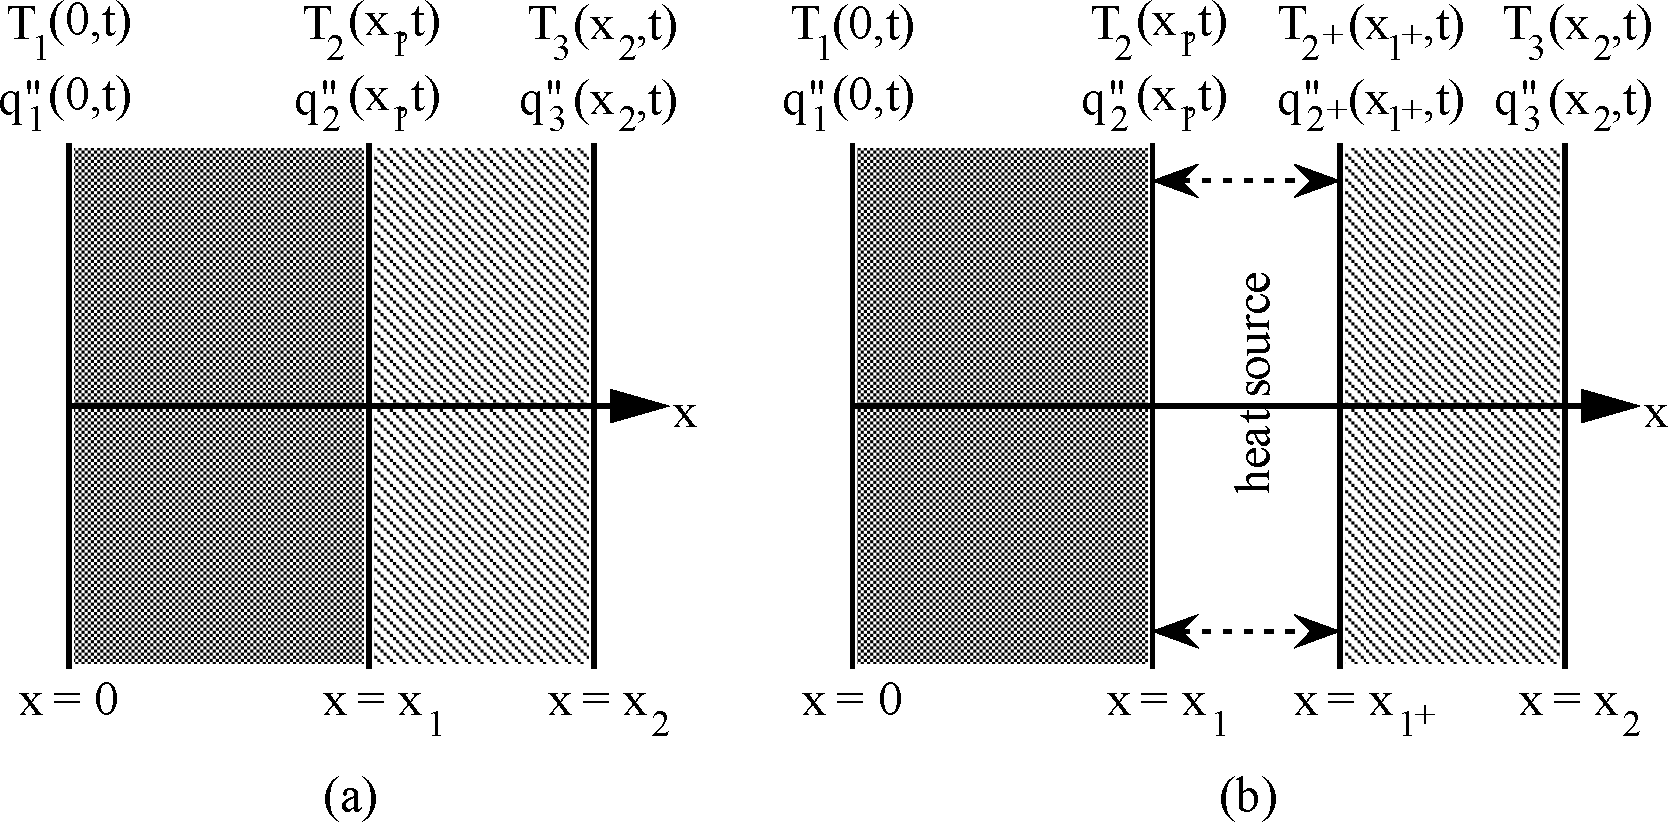
\includegraphics{media/image6009.png}
\caption{}
\end{figure}

\begin{equation}
\left[ {\begin{array}{*{20}{c}}{{T_2}\left( s \right)}\\ {{q_2}\left( s \right)}\end{array}} \right] = \left[ {\begin{array}{*{20}{c}}{{A_2}\left( s \right)}&{{B_2}\left( s \right)}\\ {{C_2}\left( s \right)}&{{D_2}\left( s \right)}\end{array}} \right]\left[ {\begin{array}{*{20}{c}}{{T_3}\left( s \right)}\\ {{q_3}\left( s \right)}\end{array}} \right]
\end{equation}

Figure 269.~ Two Layer Example for Deriving the Laplace Transform Extension to Include Sources and Sinks

For the first layer, it was determined that in the Laplace domain

\begin{equation}
\left[ {\begin{array}{*{20}{c}}{{T_1}\left( s \right)}\\ {{q_1}\left( s \right)}\end{array}} \right] = \left[ {\begin{array}{*{20}{c}}{{A_1}\left( s \right)}&{{B_1}\left( s \right)}\\ {{C_1}\left( s \right)}&{{D_1}\left( s \right)}\end{array}} \right]\left[ {\begin{array}{*{20}{c}}{{T_2}\left( s \right)}\\ {{q_2}\left( s \right)}\end{array}} \right]
\end{equation}

For the second layer:

To link the two layers and include the heat source between them, the following substitution is made:

\begin{equation}
\left[ {\begin{array}{*{20}{c}}{{T_2}\left( s \right)}\\ {{q_2}\left( s \right)}\end{array}} \right] = \left[ {\begin{array}{*{20}{c}}{{T_{2 + }}\left( s \right)}\\ {{q_{2 + }}\left( s \right)}\end{array}} \right] + \left[ {\begin{array}{*{20}{c}}0\\ {{q_{source}}\left( s \right)}\end{array}} \right]
\end{equation}

which results in:

\begin{equation}
\left[ {\begin{array}{*{20}{c}}{{T_1}\left( s \right)}\\ {{q_1}\left( s \right)}\end{array}} \right] = \left[ {\begin{array}{*{20}{c}}{{A_1}\left( s \right)}&{{B_1}\left( s \right)}\\ {{C_1}\left( s \right)}&{{D_1}\left( s \right)}\end{array}} \right]\left\{ {\left[ {\begin{array}{*{20}{c}}{{T_{2 + }}\left( s \right)}\\ {{q_{2 + }}\left( s \right)}\end{array}} \right] + \left[ {\begin{array}{*{20}{c}}0\\ {{q_{source}}\left( s \right)}\end{array}} \right]} \right\}
\end{equation}

\begin{equation}
\left[ {\begin{array}{*{20}{c}}{{T_1}\left( s \right)}\\ {{q_1}\left( s \right)}\end{array}} \right] = \left[ {\begin{array}{*{20}{c}}{{A_1}\left( s \right)}&{{B_1}\left( s \right)}\\ {{C_1}\left( s \right)}&{{D_1}\left( s \right)}\end{array}} \right]\left\{ {\left[ {\begin{array}{*{20}{c}}{{A_2}\left( s \right)}&{{B_2}\left( s \right)}\\ {{C_2}\left( s \right)}&{{D_2}\left( s \right)}\end{array}} \right]\left[ {\begin{array}{*{20}{c}}{{T_3}\left( s \right)}\\ {{q_3}\left( s \right)}\end{array}} \right] + \left[ {\begin{array}{*{20}{c}}0\\ {{q_{source}}\left( s \right)}\end{array}} \right]} \right\}
\end{equation}

\begin{equation}
\left[ {\begin{array}{*{20}{c}}{{T_1}\left( s \right)}\\ {{q_1}\left( s \right)}\end{array}} \right] = \left[ {\begin{array}{*{20}{c}}{{A_1}\left( s \right)}&{{B_1}\left( s \right)}\\ {{C_1}\left( s \right)}&{{D_1}\left( s \right)}\end{array}} \right]\left[ {\begin{array}{*{20}{c}}{{A_2}\left( s \right)}&{{B_2}\left( s \right)}\\ {{C_2}\left( s \right)}&{{D_2}\left( s \right)}\end{array}} \right]\left[ {\begin{array}{*{20}{c}}{{T_3}\left( s \right)}\\ {{q_3}\left( s \right)}\end{array}} \right] + \left[ {\begin{array}{*{20}{c}}{{A_1}\left( s \right)}&{{B_1}\left( s \right)}\\ {{C_1}\left( s \right)}&{{D_1}\left( s \right)}\end{array}} \right]\left[ {\begin{array}{*{20}{c}}0\\ {{q_{source}}\left( s \right)}\end{array}} \right]
\end{equation}

While Degiovanni concludes with this formula, some insight into what the generic equation for an element that has n layers might look like is gained by working with Equation .~ If a layer is added to the left of the first layer, the entire right hand side of Equation is multiplied by the transmission matrix of the new layer.~ Conversely, if a layer is added to the right of the second layer in Figure 269, the vector containing the Laplace transform of the temperature and heat flux at interface 3 is replaced by the product of the transmission matrix of the new layer and the vector for temperature and heat flux at the next interface, and the term dealing with the heat source is not affected.~ The general equation for a building element with n layers and m layers between the left hand surface and the heat source can be derived as:

\begin{equation}
\left[ {\begin{array}{*{20}{c}}{{T_1}\left( s \right)}\\ {{q_1}\left( s \right)}\end{array}} \right] = \left( {\prod\limits_{i = 1}^n {\left[ {\begin{array}{*{20}{c}}{{A_i}\left( s \right)}&{{B_i}\left( s \right)}\\ {{C_i}\left( s \right)}&{{D_i}\left( s \right)}\end{array}} \right]} } \right)\left[ {\begin{array}{*{20}{c}}{{T_{n + 1}}\left( s \right)}\\ {{q_{n + 1}}\left( s \right)}\end{array}} \right] + \left( {\prod\limits_{i = 1}^m {\left[ {\begin{array}{*{20}{c}}{{A_i}\left( s \right)}&{{B_i}\left( s \right)}\\ {{C_i}\left( s \right)}&{{D_i}\left( s \right)}\end{array}} \right]} } \right)\left[ {\begin{array}{*{20}{c}}0\\ {{q_{source}}\left( s \right)}\end{array}} \right]
\end{equation}

or in more compact form:

\begin{equation}
\left[ {\begin{array}{*{20}{c}}{{T_1}\left( s \right)}\\ {{q_1}\left( s \right)}\end{array}} \right] = \left[ {\begin{array}{*{20}{c}}{A\left( s \right)}&{B\left( s \right)}\\ {C\left( s \right)}&{D\left( s \right)}\end{array}} \right]\left[ {\begin{array}{*{20}{c}}{{T_{n + 1}}\left( s \right)}\\ {{q_{n + 1}}\left( s \right)}\end{array}} \right] + \left[ {\begin{array}{*{20}{c}}{a\left( s \right)}&{b\left( s \right)}\\ {c\left( s \right)}&{d\left( s \right)}\end{array}} \right]\left[ {\begin{array}{*{20}{c}}0\\ {{q_{source}}\left( s \right)}\end{array}} \right]
\end{equation}

where:~ \(\left[ {\begin{array}{*{20}{c}}{A\left( s \right)}&{B\left( s \right)}\\ {C\left( s \right)}&{D\left( s \right)}\end{array}} \right] = \prod\limits_{i = 1}^n {\left[ {\begin{array}{*{20}{c}}{{A_i}\left( s \right)}&{{B_i}\left( s \right)}\\ {{C_i}\left( s \right)}&{{D_i}\left( s \right)}\end{array}} \right]}\) ~~and~ \(\left[ {\begin{array}{*{20}{c}}{a\left( s \right)}&{b\left( s \right)}\\ {c\left( s \right)}&{d\left( s \right)}\end{array}} \right] = \prod\limits_{i = 1}^m {\left[ {\begin{array}{*{20}{c}}{{A_i}\left( s \right)}&{{B_i}\left( s \right)}\\ {{C_i}\left( s \right)}&{{D_i}\left( s \right)}\end{array}} \right]}\) ~.

Next, Equation must be rearranged to match the form of Equation , which relates the heat flux at both sides of the element to the temperature at each side.~ The matrix equation that is obtained shows that:

\begin{equation}
\left[ {\begin{array}{*{20}{c}}{{q_1}\left( s \right)}\\ {{q_{n + 1}}\left( s \right)}\end{array}} \right] = \left[ {\begin{array}{*{20}{c}}{\frac{{D\left( s \right)}}{{B\left( s \right)}}}&{\frac{{ - 1}}{{B\left( s \right)}}}\\ {\frac{1}{{B\left( s \right)}}}&{\frac{{ - A\left( s \right)}}{{B\left( s \right)}}}\end{array}} \right]\left[ {\begin{array}{*{20}{c}}{{T_1}\left( s \right)}\\ {{T_{n + 1}}\left( s \right)}\end{array}} \right] + \left[ {\begin{array}{*{20}{c}}{d\left( s \right) - \frac{{D\left( s \right)b\left( s \right)}}{{B\left( s \right)}}}\\ {\frac{{b\left( s \right)}}{{B\left( s \right)}}}\end{array}} \right]\left[ {{q_{source}}\left( s \right)} \right]
\end{equation}

This equation bears a striking resemblance to Equation .~ If the source term in Equation is dropped, then the equation is identical to Equation .~ This result conforms with the superposition principle which was used to develop the conduction transfer functions from the summation of a series of triangular pulses or ramp sets.~ Now, the effect of the heat source is simply added to the response to the temperature inputs.

While Equation is correct for any single or multilayered element, the first term in the heat source transmission matrix does not appear to match the compactness of the other terms in the matrix equation.~ It can be shown (see Strand 1995: equations 32 through 42 which detail this derivation) that the heat source transmission term for a two-layer problem reduces to

\begin{equation}
\left[ {\begin{array}{*{20}{c}}{{q_1}\left( s \right)}\\ {{q_3}\left( s \right)}\end{array}} \right] = \left[ {\begin{array}{*{20}{c}}{\frac{{D\left( s \right)}}{{B\left( s \right)}}}&{\frac{{ - 1}}{{B\left( s \right)}}}\\ {\frac{1}{{B\left( s \right)}}}&{\frac{{ - A\left( s \right)}}{{B\left( s \right)}}}\end{array}} \right]\left[ {\begin{array}{*{20}{c}}{{T_1}\left( s \right)}\\ {{T_3}\left( s \right)}\end{array}} \right] + \left[ {\begin{array}{*{20}{c}}{\frac{{{B_2}\left( s \right)}}{{B\left( s \right)}}}\\ {\frac{{{B_1}\left( s \right)}}{{B\left( s \right)}}}\end{array}} \right]\left[ {{q_{source}}\left( s \right)} \right]
\end{equation}

If this is extended to a slab with n layers and a source between the m and m+1 layers, the general matrix equation for obtaining heat source transfer functions using the Laplace transform method is:

\begin{equation}
\left[ {\begin{array}{*{20}{c}}{{q_1}\left( s \right)}\\ {{q_{n + 1}}\left( s \right)}\end{array}} \right] = \left[ {\begin{array}{*{20}{c}}{\frac{{D\left( s \right)}}{{B\left( s \right)}}}&{\frac{{ - 1}}{{B\left( s \right)}}}\\ {\frac{1}{{B\left( s \right)}}}&{\frac{{ - A\left( s \right)}}{{B\left( s \right)}}}\end{array}} \right]\left[ {\begin{array}{*{20}{c}}{{T_1}\left( s \right)}\\ {{T_{n + 1}}\left( s \right)}\end{array}} \right] + \left[ {\begin{array}{*{20}{c}}{\frac{{\bar b\left( s \right)}}{{B\left( s \right)}}}\\ {\frac{{b\left( s \right)}}{{B\left( s \right)}}}\end{array}} \right]\left[ {{q_{source}}\left( s \right)} \right]
\end{equation}

where: \(\left[ {\begin{array}{*{20}{c}}{A\left( s \right)}&{B\left( s \right)}\\ {C\left( s \right)}&{D\left( s \right)}\end{array}} \right] = \prod\limits_{i = 1}^n {\left[ {\begin{array}{*{20}{c}}{{A_i}\left( s \right)}&{{B_i}\left( s \right)}\\ {{C_i}\left( s \right)}&{{D_i}\left( s \right)}\end{array}} \right]}\) ~,

\(\left[ {\begin{array}{*{20}{c}}{a\left( s \right)}&{b\left( s \right)}\\ {c\left( s \right)}&{d\left( s \right)}\end{array}} \right] = \prod\limits_{i = 1}^m {\left[ {\begin{array}{*{20}{c}}{{A_i}\left( s \right)}&{{B_i}\left( s \right)}\\ {{C_i}\left( s \right)}&{{D_i}\left( s \right)}\end{array}} \right]}\) ~, and

\(\left[ {\begin{array}{*{20}{c}}{\bar a\left( s \right)}&{\bar b\left( s \right)}\\ {\bar c\left( s \right)}&{\bar d\left( s \right)}\end{array}} \right] = \prod\limits_{i = m + 1}^n {\left[ {\begin{array}{*{20}{c}}{{A_i}\left( s \right)}&{{B_i}\left( s \right)}\\ {{C_i}\left( s \right)}&{{D_i}\left( s \right)}\end{array}} \right]}\) ~.

At first glance, the terms in the heat source transmission matrix may appear to be reversed.~ It is expected that only the layers to the left of the source will affect q1(s), but the presence of \(\bar b\left( s \right)\) ~in the element multiplied by qsource(s) to obtain q1(s) seems to be contradictory.~ In fact, the entire term, \({{\bar b\left( s \right)} \mathord{\left/ {\vphantom {{\bar b\left( s \right)} {B\left( s \right)}}} \right. } {B\left( s \right)}}\) , must be analyzed to determine the effect of qsource(s) on q1(s).~ In essence, the appearance of \(\bar b\left( s \right)\) ~removes the effects of the layers to the right of the source from B(s) leaving only the influence of the layers to the left of the source.~ The form displayed by Equation is, however, extremely convenient because the terms in the heat source transmission matrix have the same denominators, and thus roots, as the terms in the temperature transmission matrix.~ Thus, the same roots that are calculated for the CTFs can be used for the QTFs, saving a considerable amount of computer time during the calculation of the transfer functions.

Once Equation is inverted from the Laplace domain back into the time domain, the combined CTF--QTF solution takes the following form:

\begin{equation}
{q''_{i,t}} = \sum\limits_{m = 1}^M {{X_m}{T_{i,t - m + 1}}}  - \sum\limits_{m = 1}^M {{Y_m}{T_{o,t - m + 1}}}  + \sum\limits_{m = 1}^k {{F_m}{{q''}_{i,t - m}}}  + \sum\limits_{m = 1}^M {{W_m}{q_{source,t - m + 1}}}
\end{equation}

This relation is identical to Equation except for the presence of the QTF series that takes the heat source or sink into account.

\subsubsection{State Space Formulation}\label{state-space-formulation-1}

The two-node example introduced by Seem (1987) can be utilized to examine the extension of the state space method to include heat sources or sinks.~ Figure~\ref{fig:two-node-state-space-example-with-a-heat} shows the simple two node network with a heat source added at node 1.

The nodal equations for the finite difference network shown in Figure~\ref{fig:two-node-state-space-example-with-a-heat} are:

\begin{equation}
C\frac{{d{T_1}}}{{dt}} = hA\left( {{T_o} - {T_1}} \right) + \frac{{{T_2} - {T_1}}}{R} + {q_{source}}A
\end{equation}

\begin{equation}
C\frac{{d{T_2}}}{{dt}} = hA\left( {{T_i} - {T_2}} \right) + \frac{{{T_1} - {T_2}}}{R}
\end{equation}

\begin{equation}
{q''_i} = h\left( {{T_i} - {T_2}} \right)
\end{equation}

\begin{equation}
{q''_o} = h\left( {{T_1} - {T_o}} \right)
\end{equation}

\begin{figure}[hbtp] % fig 270
\centering
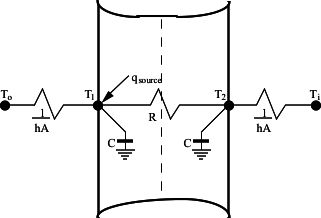
\includegraphics[width=0.9\textwidth, height=0.9\textheight, keepaspectratio=true]{media/image6034.svg.png}
\caption{Two Node State Space Example with a Heat Source \protect \label{fig:two-node-state-space-example-with-a-heat}}
\end{figure}

In obtaining the matrix equivalent for this set of equations, it should be noted that the source term is not a constant but rather an input that varies with time.~ Thus, it must be grouped with the environmental temperatures as inputs.~ The resulting matrix equations take the following form:

\begin{equation}
\left[ {\begin{array}{*{20}{c}}{\frac{{d{T_1}}}{{dt}}}\\ {\frac{{d{T_2}}}{{dt}}}\end{array}} \right] = \left[ {\begin{array}{*{20}{c}}{\frac{{ - 1}}{{RC}} - \frac{{hA}}{C}}&{\frac{1}{{RC}}}\\ {\frac{1}{{RC}}}&{\frac{{ - 1}}{{RC}} - \frac{{hA}}{C}}\end{array}} \right]\left[ {\begin{array}{*{20}{c}}{{T_1}}\\ {{T_2}}\end{array}} \right] + \left[ {\begin{array}{*{20}{c}}{\frac{{hA}}{C}}&0&{\frac{A}{C}}\\0&{\frac{{hA}}{C}}&0\end{array}} \right]\left[ {\begin{array}{*{20}{c}}{{T_o}}\\ {{T_i}}\\ {{q_{source}}}\end{array}} \right]
\end{equation}

\begin{equation}
\left[ {\begin{array}{*{20}{c}}{{{q''}_1}}\\ {{{q''}_2}}\end{array}} \right] = \left[ {\begin{array}{*{20}{c}}0&{ - h}\\h&0\end{array}} \right]\left[ {\begin{array}{*{20}{c}}{{T_1}}\\ {{T_2}}\end{array}} \right] + \left[ {\begin{array}{*{20}{c}}0&h&0\\ { - h}&0&0\end{array}} \right]\left[ {\begin{array}{*{20}{c}}{{T_o}}\\ {{T_i}}\\ {{q_{source}}}\end{array}} \right]
\end{equation}

Equation appears to suggest that the source term has no direct effect on the heat flux at either side of the element because its coefficients are zero.~ This is not the case.~ Equation only relates variables that have a direct influence on heat flux.~ So, while Ti~has no direct influence on\({q''_o}\) , it does have an indirect influence through the nodal network.~ The same would hold for the influence of qsource.

If this analysis is extended to a finite difference network with n nodes, the corresponding matrix equations can be shown to be:

\begin{equation}
\frac{{d\left[ {\begin{array}{*{20}{c}}{{T_1}}\\ \vdots \\ {{T_n}}\end{array}} \right]}}{{dt}} = \left[ A \right]\left[ {\begin{array}{*{20}{c}}{{T_1}}\\ \vdots \\ {{T_n}}\end{array}} \right] + \left[ B \right]\left[ {\begin{array}{*{20}{c}}{{T_o}}\\ {{T_i}}\\ {{q_{source}}}\end{array}} \right]
\end{equation}

\begin{equation}
\left[ {\begin{array}{*{20}{c}}{{{q''}_i}}\\ {{{q''}_o}}\end{array}} \right] = \left[ C \right]\left[ {\begin{array}{*{20}{c}}{{T_1}}\\ \vdots \\ {{T_n}}\end{array}} \right] + \left[ D \right]\left[ {\begin{array}{*{20}{c}}{{T_o}}\\ {{T_i}}\\ {{q_{source}}}\end{array}} \right]
\end{equation}

The influence of the heat source is also confirmed by the final solution form, which is identical to the Laplace transform result shown in Equation .~ As with the Laplace solution method, the state space method results in a set of QTFs that relate the heat source at the current time step and several previous time steps to the current heat flux at the surface of the element.

Other similarities between the two solution methods are evident.~ It is interesting to note that as with the Laplace method there is no alteration of the CTFs calculated by the state space method.~ Thus, the principle of superposition is still valid.~ Furthermore, the introduction of the source term did not substantially increase the computing effort required to calculate the additional transfer functions.~ In the Laplace method, this was shown by the common roots, B(s), shared by both the CTFs and the QTFs.~ In the state space method, it can be noted that the A matrices in Equations and are identical.~ Since the state space method requires the inversion and the exponentiation of the A matrix only, the additional QTF terms will not require a substantial amount of additional computing time for their calculation.

\subsubsection{Determination of Internal Temperatures}\label{determination-of-internal-temperatures}

One aspect of low temperature radiant systems that has not been addressed to this point is the appropriateness of specifying the effect of the system on slab response via a heat source term.~ For a heating system that employs electrical resistance heating, the use of a heat source as the input variable is logical.~ The heat produced by such a system can easily be related to the current passing through the heating wire.~ However, for a hydronic heating or cooling system, the known quantity is not heat but rather the temperature of the water being sent to the building element.

The use of a temperature to simulate the presence of a heating or cooling system presents one major obstacle.~ When fluid is not being circulated, there is no readily available temperature value available for use as an input variable.

In a hydronic system, a link between the fluid temperature being sent to the slab and the heat delivered to the slab exist.~ The most effective way of relating these two variables is to consider the slab to be a heat exchanger.~ Using heat exchanger relationships, an equation could then be formulated to obtain the heat delivered to the slab based on the inlet fluid temperature.

Most heat exchangers are used to thermally link two fluids.~ In the case of a hydronic radiant system, there is only one fluid and a stationary solid.~ Presumably, if the inlet fluid temperature, the system geometry, and the solid temperature are known, then the outlet temperature and thus the heat transfer to the building element can be computed.~ This leads to an interesting question:~ what is the solid temperature?

By definition, for one dimensional conduction heat transfer, the solid temperature is the temperature of the building element at the depth where the hydronic loop is located.~ Typically, this temperature is not known because it is not needed.~ The goal of both methods of calculating CTFs was the elimination of internal temperatures that were not needed for the simulation.~ For a hydronic system, it is necessary to extract this information to solve for the heat source term.~ Two methods of accomplishing this are described below.

Returning to the two layer example shown in Figure 269, it can be shown that the final solution form in the time domain for the slab with a source at the interface between the two layers is:

\begin{equation}
{q''_{1,t}} = \sum\limits_{m = 1}^M {{X_{k,m}}{T_{1,t - m + 1}}}  - \sum\limits_{m = 1}^M {{Y_{k,m}}{T_{3,t - m + 1}}}  + \sum\limits_{m = 1}^k {{F_m}{{q''}_{1,t - m}}}  + \sum\limits_{m = 1}^M {{W_m}{q_{source,t - m + 1}}}
\end{equation}

A similar equation could be written for the response of the first layer in absence of any source term and is given by:

\begin{equation}
{q''_{1,t}} = \sum\limits_{m = 1}^M {{x_{k,m}}{T_{1,t - m + 1}}}  - \sum\limits_{m = 1}^M {{y_{k,m}}{T_{2,t - m + 1}}}  + \sum\limits_{m = 1}^k {{f_m}{{q''}_{1,t - m}}}
\end{equation}

While the current temperature at the interface is not known, presumably the previous values of this parameter will be known.~ In addition, the temperatures and the flux histories at surface 1 are also know.~ The unknowns in Equation are the current heat flux at surface 1 and the temperature at surface 2.~ However, Equation does define the current value of the heat flux at surface 1 based on temperature, heat flux, and heat source histories.~ Thus, if this value is used in Equation , the only remaining unknown in this equation is the current temperature at surface 2, the surface where the heat source or sink is present.~ Rearranging Equation provides an equation from which the temperature at the source location may be calculated:

\begin{equation}
{T_{2,t}} = \sum\limits_{m = 1}^M {{{\bar X}_{k,m}}{T_{1,t - m + 1}}}  - \sum\limits_{m = 1}^{M - 1} {{{\bar Y}_{k,m}}{T_{2,t - m}}}  + \sum\limits_{m = 1}^{k + 1} {{{\bar F}_m}{{q''}_{1,t - m + 1}}}
\end{equation}

where the new coefficients are obtained from the standard conduction transfer functions for the first layer via the following equations:

\begin{equation}
{\bar X_{k,m}} = \frac{{{x_{k,m}}}}{{{y_1}}}\left( {m = 1, \cdots ,M} \right)
\end{equation}

\begin{equation}
{\bar Y_{k,m}} = \frac{{{y_{k,m + 1}}}}{{{y_1}}}\left( {m = 1, \cdots ,M - 1} \right)
\end{equation}

\begin{equation}
{\bar F_1} = \frac{1}{{{y_1}}}
\end{equation}

\begin{equation}
{\bar F_m} = \frac{{{f_{m - 1}}}}{{{y_1}}}\left( {m = 2, \cdots ,k + 1} \right)
\end{equation}

This system for backing out an internal temperature through the use of a second, rearranged CTF equation is valid regardless of whether the Laplace transform or state space method is utilized to calculate the CTFs and QTFs.~ The state space method, however, offers a more direct method of obtaining an internal temperature through its definition as an additional output variable.

Consider again the state space example shown in Figure~\ref{fig:two-node-state-space-example-with-a-heat}.~ Two output variables were defined for this example: \({q''_i}\) ~and \({q''_o}\) .~ The temperature of the node where the source is present can also be defined as an output variable through the identity equation:

\begin{equation}
{T_1} = {T_1}
\end{equation}

When this equation for T1~is added to Equation , the resulting output matrix equation for the heat flux at both surfaces and the internal temperature is:

\begin{equation}
\left[ {\begin{array}{*{20}{c}}{{{q''}_i}}\\ {{{q''}_o}}\\ {{T_1}}\end{array}} \right] = \left[ {\begin{array}{*{20}{c}}0&{ - h}\\h&0\\1&0\end{array}} \right]\left[ {\begin{array}{*{20}{c}}{{T_1}}\\ {{T_2}}\end{array}} \right] + \left[ {\begin{array}{*{20}{c}}0&h&0\\ { - h}&0&0\\0&0&0\end{array}} \right]\left[ {\begin{array}{*{20}{c}}{{T_i}}\\ {{T_o}}\\ {{q_{source}}}\end{array}} \right]
\end{equation}

The only difference between this relation and Equation is the presence of T1~on both the right and left hand side of the equation.~ The dual role of T1~as a state variable and an output parameter may seem to contradict the goal of the state space method of eliminating the state variables.~ However, due to the flexibility of the formulation, nodal temperatures can be extracted in the same manner that any other output quantity would be obtained.~ For an element with n layers, Equation becomes:

\begin{equation}
\left[ {\begin{array}{*{20}{c}}{{{q''}_i}}\\ {{{q''}_o}}\\ {{T_s}}\end{array}} \right] = \left[ C \right]\left[ {\begin{array}{*{20}{c}}{{T_1}}\\ \vdots \\ {{T_n}}\end{array}} \right] + \left[ D \right]\left[ {\begin{array}{*{20}{c}}{{T_i}}\\ {{T_o}}\\ {{q_{source}}}\end{array}} \right]
\end{equation}

where Ts~is the temperature of the node where the heat source or sink is present.~ The transfer function equation for the calculation of Ts~that results from Equation is identical in form to Equation :

\begin{equation}
{T_{s,t}} = \sum\limits_{m = 1}^M {{x_{k,m}}{T_{i,t - m + 1}}}  - \sum\limits_{m = 1}^M {{y_{k,m}}{T_{o,t - m + 1}}}  + \sum\limits_{m = 1}^k {{f_m}{T_{s,t - m}}}  + \sum\limits_{m = 1}^M {{w_m}{q_{source,t - m + 1}}}
\end{equation}

Instead of the flux at either side of the element characterized as a function of temperature, flux, and source history terms, the temperature at the source location is related to source and temperature histories including histories of Ts.~ The validity of these internal temperature calculation methods as well as heat source transfer functions in general will be discussed in the next chapter.

\subsubsection{Low Temperature Radiant System Controls}\label{low-temperature-radiant-system-controls}

The use of this equation allows the low temperature radiant system to be handled like any other surface within the heat balance framework.~ Heat balances at the inside and outside surfaces take on the same form as other surfaces, and the participation of the radiant system in the radiation balance within the space and thermal comfort models is automatically included.~ Thus, the radiant system model is fully integrated into the heat balance, and any improvements that are made in areas such as convection coefficients, shading models, etc. are immediately available to the radiant system as part of the overall heat balance solution.

Once the transient nature of the system is accounted for, one must then turn to the next difficult issue: controls.~ Controls are problematic for almost any simulation program.~ The problem is not whether something can be simulated because typically a simulation program offers the ability to experiment with many different control strategies.~ Rather, the problem is typically the diversity of controls that are implemented and keeping the controls that can be simulated up to date.~ EnergyPlus offers two different control schemes: variable flow (ZoneHVAC:LowTemperatureRadiant:VariableFlow) and variable temperature (ZoneHVAC:LowTemperatureRadiant:ConstantFlow).~ The control strategies are different enough that they were developed as separate system types.~ More details of the controls are described below.

The controls for variable flow low temperature radiant systems within EnergyPlus are fairly simple though there is some flexibility through the use of schedules.~ The program user is allowed to define a setpoint temperature as well as a throttling range through which the system varies the flow rate of water (or current) to the system from zero to the user defined maximum flow rate.~ The flow rate is varied linearly with the flow reaching 50\% of the maximum when the controlling temperature reaches the setpoint temperature.~ Setpoint temperatures can be varied on an hourly basis throughout the year if desired.~ The controlling temperature can be the mean air temperature, the mean radiant temperature, or the operative temperature of the zone, and this choice is also left to the user's discretion.~ (Operative temperature for radiant system controls is the average of MAT and MRT.)~ Since flow rate is varied, there is no explicit control on the inlet water temperature or mixing to achieve some inlet water temperature in a hydronic system.~ However, the user does have the ability to specify on an hourly basis through a schedule the temperature of the water that would be supplied to the radiant system.

Graphical descriptions of the controls for the low temperature radiant system model in EnergyPlus are shown in Figure~\ref{fig:variable-flow-low-temperature-radiant-system} for a hydronic system.~ In a system that uses electric resistance heating, the power or heat addition to the system varies in a manner similar to mass flow rate variation shown in Figure~\ref{fig:variable-flow-low-temperature-radiant-system}.

In the constant flow-variable temperature systems, the controls are also considered piecewise linear functions, but in this case the user selects both the control temperatures and the water temperatures via schedules.~ This offers greater flexibility for defining how the radiant system operates though it may not model every situation.~ Figure~\ref{fig:variable-temperature-low-temperature-radiant} shows how the ``desired'' inlet water temperature is controlled based on user schedules.~ The user has the ability to specify the high and low water and control temperature schedules for heating and cooling (separately; a total of eight temperature schedules).~ Note that this inlet temperature is a ``desired'' inlet temperature in that there is no guarantee that the system will provide water to the system at that temperature.~ The model includes a local loop that attempts to meet this demand temperature through mixing and recirculation.

\begin{figure}[hbtp] % fig 271
\centering
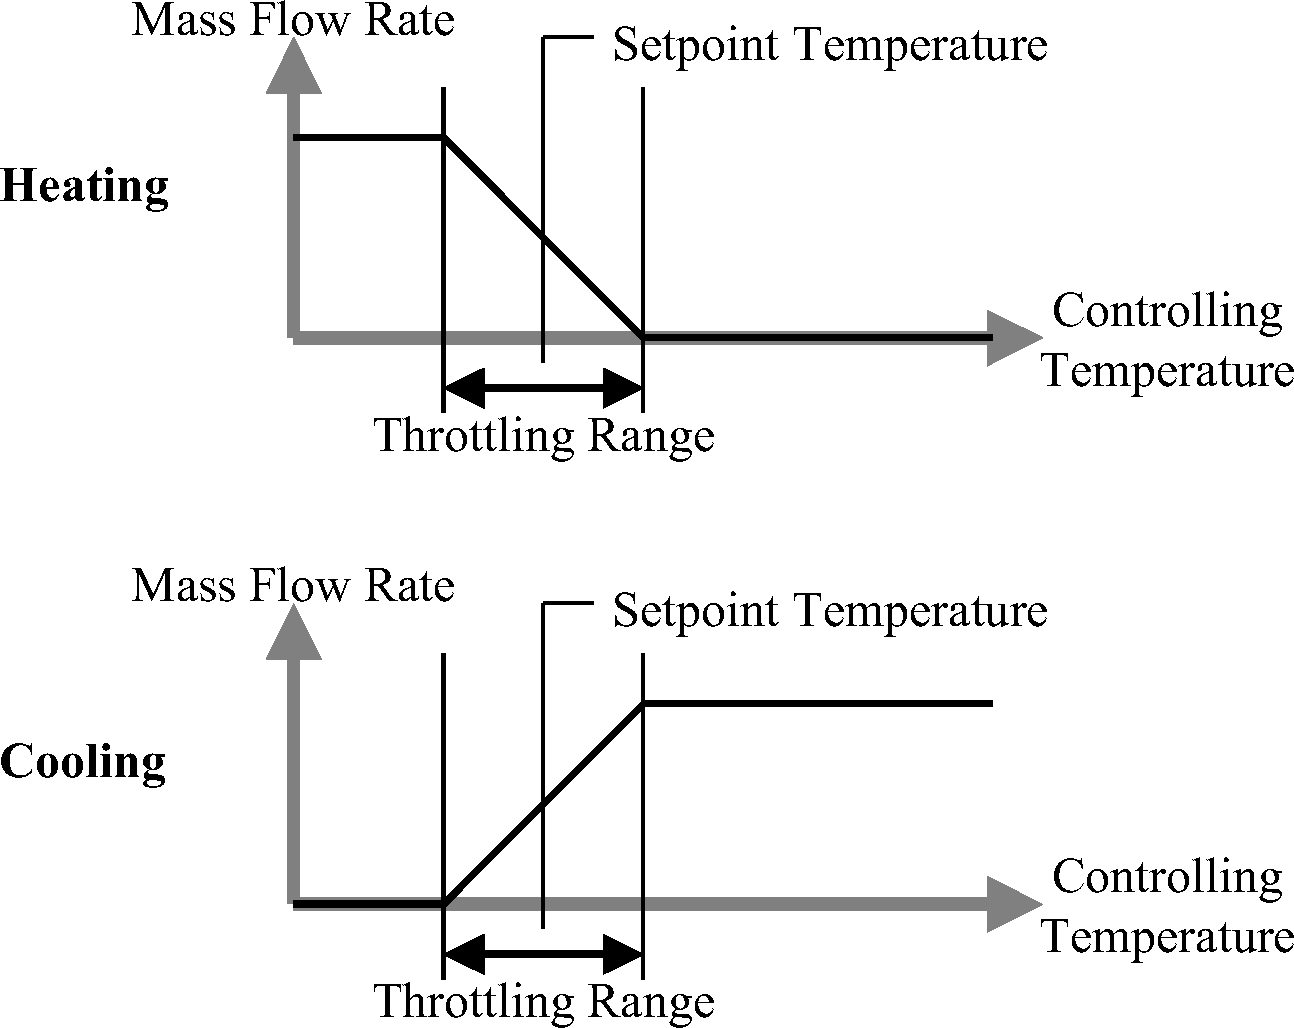
\includegraphics[width=0.9\textwidth, height=0.9\textheight, keepaspectratio=true]{media/image6053.png}
\caption{Variable Flow Low Temperature Radiant System Controls \protect \label{fig:variable-flow-low-temperature-radiant-system}}
\end{figure}

\begin{figure}[hbtp] % fig 272
\centering
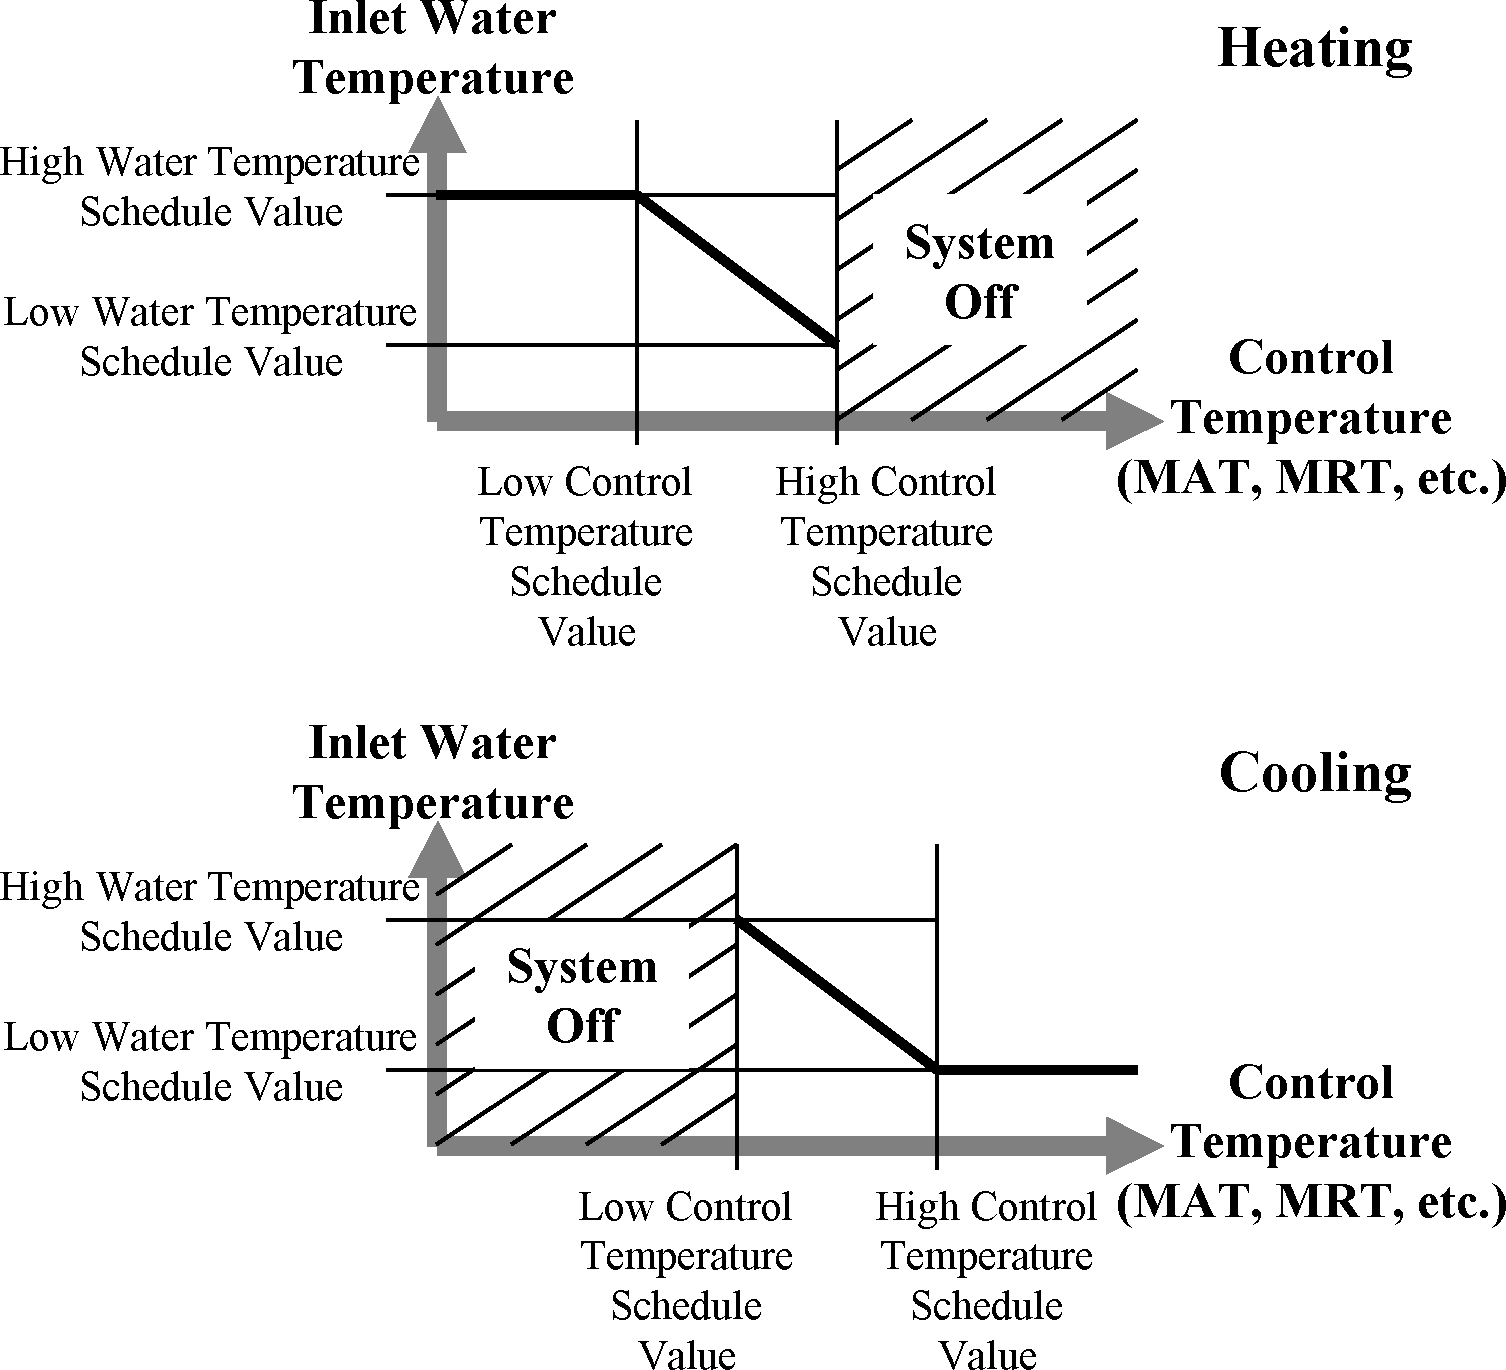
\includegraphics[width=0.9\textwidth, height=0.9\textheight, keepaspectratio=true]{media/image6054.png}
\caption{Variable Temperature Low Temperature Radiant System Controls \protect \label{fig:variable-temperature-low-temperature-radiant}}
\end{figure}

The constant flow (variable temperature) low temperature radiant system model is actually a combination of mixing valves, a pump (constant speed, but the maximum flow can be modified by a schedule), and the radiant system (surface, panel, or group of surfaces/panels).~ This is connected to the main loop through the standard inlet connections as shown in Figure~\ref{fig:variable-temperature-low-temperature-radiant-001}.~ The system controls determine the desired inlet temperature and system flow rate while loop controls determine the flow rate and temperature of the loop.~ Note that pump heat also factors into the model through a simple constant speed pump model and user input.

There are four possible conditions (separate for heating and cooling).~ First, if the loop has adequate temperature and flow to meet system requests, then the model sets the radiant system inlet temperature and controls to the desired values based on the controls and simulates.~ This is the best condition and recirculation and bypass amounts are adjusted accordingly based on radiant system outlet temperatures.~ Second, if the loop temperature is adequate but the loop flow rate is less than the radiant system flow rate, we may or may not be able to meet the desired inlet temperature since recirculation might lower the temperature below the desired temperature.~ In this second case, the model first simulates the radiant system with the desired conditions and then resimulates it to solve for the actual inlet temperature (see later in this section) if it cannot achieve the desired inlet temperature.~ Third, if the loop flow is greater than the radiant flow but the temperature of the loop is not adequate, then there is no amount of mixing that will solve this problem.~ All of the radiant flow comes from the loop and the loop temperature (after pump heat addition) becomes the radiant system inlet regardless of the temperature controls.~ Finally, if both the temperature and the flow of the loop are inadequate, then the model simply solves for the actual radiant system inlet temperature and does not try to meet the controls (merely tries to get as close as physically possible given the loop conditions).

\begin{figure}[hbtp] % fig 273
\centering
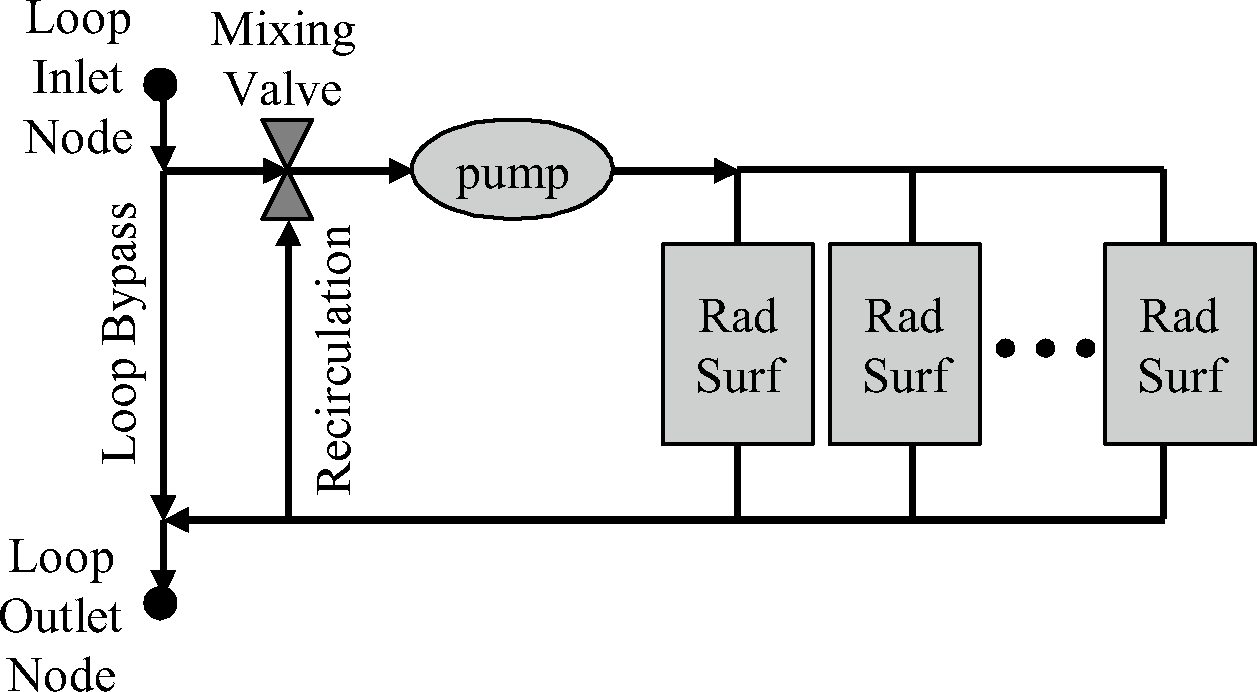
\includegraphics[width=0.9\textwidth, height=0.9\textheight, keepaspectratio=true]{media/image6055.png}
\caption{Variable Temperature Low Temperature Radiant System Component Details \protect \label{fig:variable-temperature-low-temperature-radiant-001}}
\end{figure}

One remaining challenge is the merging of the low temperature radiant system model with an integrated building simulation program.~ In the past, most simulation programs have simulated the building envelope, the space conditioning systems, and the central plant equipment in three separate steps.~ While this had some advantages and was partly due to a lack of computing capacity, the large drawback for this arrangement is that there is no feedback from the space conditioning system or central plant response to the building conditions.~ Thus, if the system or plant was undersized, it was reported as an ``unmet load'' and does not affect the temperatures experienced within the building.~ IBLAST, a predecessor (Taylor 1991) to EnergyPlus, resolved this issue by integrating all three major components of a building simulation and thus allowing feedback between the equipment and the building envelope.

This integration was not a trivial task and required that the systems be simulated at shorter time steps in some cases to maintain solution stability.~ In essence, the system simulation will shorten its time step whenever it senses that conditions are changing too rapidly.~ While this is effective in maintaining solution stability, it can present problems for a radiant system.~ The radiant system has either a direct or an indirect impact on the surfaces within a building.~ So, it must be simulated with the building envelope.~ Yet, it is also a space conditioning system that must act on the space like any other system and thus must also be simulated at the system time step, which can be less than the building time step and can also vary within EnergyPlus.

This issue was handled using a multi-step approach.~ In EnergyPlus, the heat balance is always simulated first.~ When this happens, the radiant system is temporarily shut-off to find how the building would respond if there was no heat source/sink.~ Then, as the system and plant are simulated at multiple shorter time steps, the radiant system is allowed to operate per the controls specified by the user.~ Flow rate is allowed to vary at each system time step, and the radiant system model is simulated at each time step as if the current flow rate was being used throughout the entire zone time step.~ This means that each time the heat source/sink in the radiant system is varied during the system simulation the zone heat balance must be recomputed to see what the reaction of the rest of the zone is to this change in the conditions of one (or more) of the surfaces.

In reality, this is not physically correct because each change in the flow rate throughout the system simulation will have an impact on the system time steps remaining before the heat balance is simulated during the next zone time step.~ Yet, other approaches to solving the mismatch between the system and the zone response of radiant systems are not feasible.~ One could force the system to run at the same time step as the zone, but this could result in instabilities in other types of systems that might be present in the simulation.~ On the other hand, one could try to force the zone to run at the shorter time steps of the system, but this could lead to instability within the heat balance due to limits on the precision of the conduction transfer function coefficients.

Despite the fact that the simulation algorithm described above may either over- or under-predict system response dependent on how the system has been controlled in previous system time steps, it is reasonable to expect that the effect of these variations will balance out over time even though it might lead to slightly inaccurate results at any particular system time step.~ The long-term approach is also in view in the final simulation step at each zone time step.~ After the system has simulated through enough system time steps to equal a zone time step, the radiant system will rerun the heat balance using the average heat source/sink over all of the system time steps during the past zone time step.~ This maintains the conservation of energy within the heat balance simulation over the zone time steps and defines more appropriate temperature and flux histories at each surface that are critical to the success of a conduction transfer function based solution.~ A graphical picture of this somewhat complex multiple step simulation is shown in the figure below.

\begin{figure}[hbtp] % fig 274
\centering
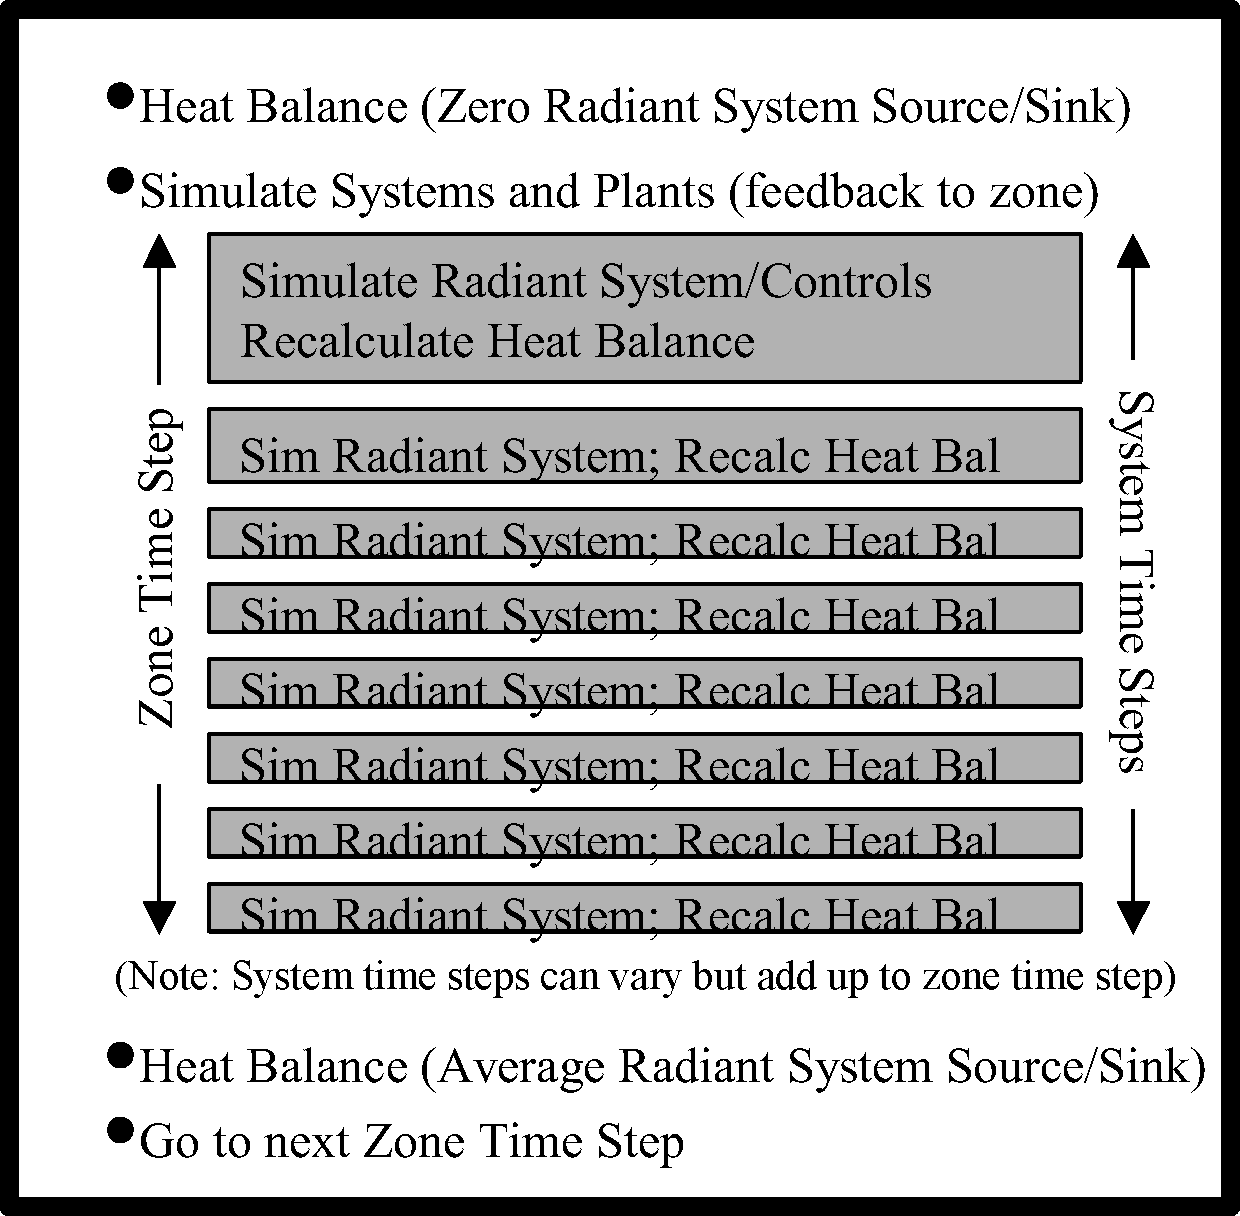
\includegraphics[width=0.9\textwidth, height=0.9\textheight, keepaspectratio=true]{media/image6056.png}
\caption{Resolution of Radiant System Response at Varying Time Steps \protect \label{fig:resolution-of-radiant-system-response-at}}
\end{figure}

\subsubsection{Heat Exchanger Formulation for Hydronic Systems}\label{heat-exchanger-formulation-for-hydronic-systems}

As has been mentioned previously, the actual heat transferred between the building element and the hydronic loop is related to the temperature of the building element at the source location as well as the water system inlet and outlet temperatures.~ In EnergyPlus, it is assumed that the inlet temperature to the slab (defined by a user schedule and the plant simulation) and the mass flow rate (determined by the control algorithm) are known and that the remaining parameters must be calculated.~ However, the heat balance equations require the heat transferred to the building element from the water loop in order to calculate the heat transferred from the element to the building environment.

Even though systems defined by this model can vary somewhat, the same characteristic link between the system variables exist.~ For modeling purposes, the overall water/slab system can be thought of as a heat exchanger.~ While in principle there are two alternative heat exchanger methodologies, it is more convenient to use the effectiveness-NTU method in this case.

Several assumptions will be incorporated into the heat exchanger analysis.~ It is assumed that the building element that contains the hydronic loop is stationary and that its temperature along the length of the tubing is constant.~ The latter part of this assumption stems from assumptions made in both the one and two dimensional heat source transfer function derivations.~ In either case, the source was added at a single node that was characterized by a single temperature.~ For consistency, this assumption must be made again in the heat exchanger analysis.~ Another assumption for the current EnergyPlus model is that the fluid in the tubing is water.~ Additionally, it is assumed that the thermal properties of the water do not vary significantly over the length of the tubing and that the water flows at a constant flow rate.~ Finally, the temperature at the inside surface of the water tubing is assumed to be equal to the temperature at the source location.~ In other words, it is assumed that the water tubing itself has no appreciable effect on the heat transfer process being modeled.

Using these assumptions and the effectiveness-NTU heat exchanger algorithm, several equations can be defined which establish the relationship between the heat source and the water temperatures.~ First, a heat balance on the water loop results in:

\begin{equation}
q = {\left( {\dot m{c_p}} \right)_{water}}\left( {{T_{wi}} - {T_{wo}}} \right)
\end{equation}

where q is the energy transferred between the water loop and the building element, \(\dot m\) ~is the mass flow rate of the water, cp~is the specific heat of the water, Twi~is the inlet water temperature, and Two~is the outlet water temperature.

The maximum amount of heat transfer that is possible according to the Second Law of Thermodynamics is:

\begin{equation}
{q_{\max }} = {\left( {\dot m{c_p}} \right)_{water}}\left( {{T_{wi}} - {T_s}} \right)
\end{equation}

where qmax~is the maximum amount of energy transfer that is possible and Ts~is the temperature at the source location.

The effectiveness of the heat exchanger, e, is defined as the ratio of the actual energy transfer to the maximum possible, or:

\begin{equation}
\varepsilon  \equiv \frac{q}{{{q_{\max }}}}
\end{equation}

For a heat exchanger where one fluid is stationary, the effectiveness can be related to NTU, the number of transfer units, by the following equation (Incropera and DeWitt 1985):

\begin{equation}
\varepsilon  = 1 - {e^{ - NTU}}
\end{equation}

where NTU is defined by:

\begin{equation}
NTU \equiv \frac{{UA}}{{{{\left( {\dot m{c_p}} \right)}_{water}}}}
\end{equation}

Since the water tubes were assumed to have no effect on the heat transfer process, the only term present in the overall heat transfer coefficient, UA, is a convection term.~ Thus, the equation for UA is:

\begin{equation}
UA = h\left( {\pi DL} \right)
\end{equation}

where h is the convection coefficient, D is the interior tube diameter, and L is the total length of the tube.

The convection coefficient can be obtained from internal flow correlations that relate the Nusselt dimensionless number to other flow properties.~ For laminar flow in a tube of constant surface temperature, the Nusselt number is defined by:

\begin{equation}
N{u_D} = \frac{{hD}}{k} = 3.66
\end{equation}

where k is the thermal conductivity of the water.

For turbulent internal flow, the Colburn equation can be used to define the Nusselt number:

\begin{equation}
N{u_D} = \frac{{hD}}{k} = 0.023{\mathop{\rm Re}\nolimits}_D^{{4 \mathord{\left/ {\vphantom {4 5}} \right. } 5}}{\Pr ^{{1 \mathord{\left/ {\vphantom {1 3}} \right. } 3}}}
\end{equation}

where Pr is the Prandtl number of water and ReD~is the Reynolds number which is defined by:

\begin{equation}
{{\mathop{\rm Re}\nolimits}_D} = \frac{{4\dot m}}{{\pi \mu D}}
\end{equation}

The parameter m is the absolute viscosity of water.~ For internal pipe flow, the flow is assumed to be turbulent for ReD~≥ 2300.

Knowledge of the flow conditions allows Equations through to be calculated.~ This essentially eliminates e as an unknown in Equation .~ The controls and the plant define the water mass flow rate and the inlet water temperature, leaving two equations (Equations and ) and three unknowns.~ The third equation that can be used in conjunction with Equations and is Equation , which is the CTF/QTF equation for the temperature at the source location.

Knowing the inlet water temperature and water mass flow rate, the calculation procedure is somewhat involved and requires, in addition to Equations , , and , the use of a modified form of Equation .~ Equation is the standard conduction transfer function formula for a building element with an embedded source/sink of heat.~ In EnergyPlus, the surface flux on the left hand side of the equation is replaced with a surface heat balance:

\begin{equation}
\left[ {\begin{array}{*{20}{c}}{Surface}\\ {Heat}\\ {Balance}\end{array}} \right] = \sum\limits_{m = 1}^M {{X_{k,m}}{T_{1,t - m + 1}}}  - \sum\limits_{m = 1}^M {{Y_{k,m}}{T_{3,t - m + 1}}}  + \sum\limits_{m = 1}^k {{F_m}{{q''}_{1,t - m}}}  + \sum\limits_{m = 1}^M {{W_m}{q_{source,t - m + 1}}}
\end{equation}

The surface heat balance includes terms for incident solar energy, radiation heat transfer from internal heat sources such as lights and electrical equipment, radiation between surfaces using Hottel's Gray Interchange concept, and convection to the surrounding air.~ The presence of the surface temperature in the heat balance does not pose any problems since Equation will be rearranged to solve for this temperature.~ Since the radiation heat balance is dependent on conditions at the other surfaces, an iteration loop is required to provide a more accurate estimate of the radiative exchange within the building.~ This is not the case with the mean air temperature.~ An assumption of the heat balance is that the mean temperature of the surrounding air is equal to the final air temperature of the previous time step.~ Using this estimate in the heat balance avoids a second iterative loop around the radiative iteration loop.

Thus, the terms of the heat balance on the left hand side of the equation have been set with the only unknown quantity being Ti, the inside surface temperature at the current time step.~ On the right hand side of Equation , most of the terms are already defined since they depend on known values from previous time steps (temperature, flux, and source histories).~ The only terms which are not defined are the inside surface temperature (Ti), outside surface temperature (To), and internal heat source/sink (qsource) of the current time step.

The outside surface temperature will depend on the type of environment to which it is exposed.~ For example, if the surface is a slab on grade floor, the outside surface temperature is defined as ground temperature and does not require an outside surface heat balance.~ If the element is an interior surface which has both surfaces exposed to the same air space, the outside surface temperature is redefined to be equal to the inside surface temperature.~ In cases where the outside surface temperature is not simply defined such as a surface exposed to the exterior environment, a heat balance similar to Equation is required to define the outside surface temperature.~ However, to again avoid iteration, the heat balance equation for the outside surface assumes that conditions at the inside surface were the same as the previous time step.~ In most cases, since the influence of the current inside surface temperature on the outside surface temperature is very small, this is a valid assumption.~ In cases were the inside surface temperature has a significant effect, an approximate inside surface heat balance which defines the inside surface temperature is used.~ This approximate inside balance uses mean air and radiant temperatures from the previous time step.

At this point in the simulation algorithm then, all of the terms in Equation have been defined except the value at the current time step of the inside surface temperature and the heat source/sink.~ Thus, Equation can be rewritten in a simpler form:

\begin{equation}
{T_{i,t}} = {C_1} + {C_2}{q_{source,t}}
\end{equation}

where the variable C1~includes surface heat balance and past history terms as well as the influence of the current outside temperature.~ The term C2~will depend on the heat source transfer function term and the coefficients of terms linked directly to Ti,t.

Equation , which was the CTF/QTF equation for the temperature at the source location, can be simplified in a similar manner.~ Grouping the temperature and source history terms which are known quantities together with the effect of the outside surface temperature which is defined as described above, the original equation

\begin{equation}
{T_{s,t}} = \sum\limits_{m = 1}^M {{x_{k,m}}{T_{i,t - m + 1}}}  - \sum\limits_{m = 1}^M {{y_{k,m}}{T_{o,t - m + 1}}}  + \sum\limits_{m = 1}^k {{f_m}{T_{s,t - m}}}  + \sum\limits_{m = 1}^M {{w_m}{q_{source,t - m + 1}}}
\end{equation}

can be reduced to:

\begin{equation}
{T_s} = {C_3} + {C_4}{q_{source,t}} + {C_5}{T_{i,t}}
\end{equation}

where C3~includes all of the history terms and the effect of the current outside temperature, C4~is the heat source transfer function for the current time step, and C5~is the conduction transfer function for the inside surface temperature at the current time step.

Substituting Equation into Equation and noting that qsource,t~is the same quantity as q in Equations and results in:

\begin{equation}
{T_s} = {C_3} + {C_4}q + {C_5}\left( {{C_1} + {C_2}q} \right)
\end{equation}

When this equation is combined with Equation , the heat source, which results from a known water inlet temperature, can be shown to be:

\begin{equation}
q = \frac{{{T_{wi}} - {C_3} - {C_1}{C_5}}}{{\frac{1}{{\varepsilon {{\left( {\dot m{c_p}} \right)}_{water}}}} + {C_4} + {C_2}{C_5}}}
\end{equation}

With both q and Twi~known, it is a trivial matter to calculate Two~and Ts~from Equations and , respectively.~ Even though the coefficients in Equation are fairly complex, the final equation relating the heat source directly to inlet water temperature is compact and does not require any iteration.~ As with flux control, once the heat source/sink is defined, the inside surface heat balance can be performed to determine the surface temperatures.

It should be noted that Equations through are a slight simplification of the actual implementation in EnergyPlus.~ The development shown above follows the heat balance conventions that assume previous values of the inside temperature to calculate the outside temperature.~ This, in reality, is not necessary and since the radiant system can be significantly influenced by the delay that such an assumption might cause, the initial implementation of radiant systems in EnergyPlus used a development (shown below) that does not lag either the inside or the outside surface temperature.~ In effect, we can establish three basic equations for the temperature at the inside and outside surface as well as at the location of the heat source/sink:

\begin{equation}
{T_{inside}} = {C_a} + {C_b}{T_{outside}} + {C_C}q''
\end{equation}

\begin{equation}
{T_{outside}} = {C_d} + {C_e}{T_{inside}} + {C_f}q''
\end{equation}

\begin{equation}
{T_{source}} = {C_g} + {C_h}q'' + {C_i}{T_{inside}} + {C_j}{T_{outside}}
\end{equation}

where: T\(_{inside}\) is the temperature at the inside surface

T\(_{outside}\) is the temperature at the outside surface

T\(_{source}\) is the temperature within the radiant system at the location of the source/sink

C\(_{a}\) is all of the other terms in the inside heat balance (solar, LW exchange, conduction history terms, etc.)

C\(_{b}\) is the current cross CTF term

C\(_{c}\) is the QTF inside term for the current heat source/sink

C\(_{d}\) is all of the other terms in the outside heat balance (solar, LW exchange, conduction history terms, etc.)

C\(_{e}\) is the current cross CTF term (should be equal to Cb)

C\(_{f}\) is the QTF outside term for the current heat source/sink

C\(_{g}\) is the summation of all temperature and source history terms at the source/sink location

C\(_{h}\) is the QTF term at the source/sink location for the current heat source/sink

C\(_{i}\) is the CTF inside term for the current inside surface temperature

C\(_{j}\) is the CTF outside term for the current outside surface temperature

Equations and above can be solved to remove the other surface temperature. Substituting the new equations for T\(_{inside}\) and T\(_{outside}\) as a function of C and q" into the equation for Tsource and simplifying results in the following equation:

\begin{equation}
{T_{source}} = {C_k} + {C_l}q''
\end{equation}

where:~~~~~~~~ \({C_k} = {C_g} + \frac{{{C_i}\left( {{C_a} + {C_b}{C_d}} \right) + {C_j}\left( {{C_d} + {C_e}{C_a}} \right)}}{{1 - {C_e}{C_b}}}\)

\begin{equation}
{C_l} = {C_h} + \frac{{{C_i}\left( {{C_c} + {C_b}{C_f}} \right) + {C_j}\left( {{C_f} + {C_e}{C_c}} \right)}}{{1 - {C_e}{C_b}}}
\end{equation}

Combining this with heat exchanger analysis as shown above, we eventually arrive at the following equation to relate the flux to the slab to the water inlet temperature and mass flow rate:

\begin{equation}
q'' = \frac{{{T_{water,in}} - {C_k}}}{{\frac{{{C_l}}}{A} + \frac{1}{{\varepsilon {{\left( {\dot m{c_p}} \right)}_{water}}}}}}
\end{equation}

which includes all of the inside and outside heat balance terms (``hidden'' in the C\(_{k}\) and C\(_{l}\) coefficients).~ Once the flux to the slab is known, the remaining terms of interest (outlet water temperature, inside and outside surface temperatures, etc.) can be calculated using the relatively simpler equations shown above.

Note that the above development is valid for both the hydronic (variable flow) low temperature radiant system and for constant flow (variable temperature) low temperature radiant systems where the inlet temperature is known (based on controls).~ However, when due to loop conditions and the presence of recirculation, it is not possible to know the inlet temperature to the radiant system without simulating it, we must either iterate or perform more mathematics to arrive at the inlet temperature.~ The implementation in EnergyPlus chose to avoid iteration and solved for the inlet temperature as shown in the next paragraphs.

The previous equation combines with the following equation which is valid for an surface in the current radiant system:

\begin{equation}
{{\rm{q}}_{\rm{j}}}{\rm{  =  }}{{\rm{\dot m}}_{\rm{j}}}{{\rm{c}}_{\rm{p}}}{\rm{(}}{{\rm{T}}_{{\rm{water,in}}}}{\rm{  -  }}{{\rm{T}}_{{\rm{water,out,j}}}}{\rm{)}}
\end{equation}

where q\(_{j}\) is the heat transfer to the jth surface in the radiant system, m\(_{j}\) is the mass flow rate only to this surface, and T\(_{water,out,j}\) is the outlet temperature for the jth surface.~ Combining the previous two equations results in:

\begin{equation}
{\rm{(}}{{\rm{T}}_{{\rm{water,in}}}}{\rm{  -  }}{{\rm{T}}_{{\rm{water,out,j}}}}{\rm{)}} = \frac{{{\varepsilon_j}\left( {{{\rm{T}}_{{\rm{water,in}}}} - {C_{k,j}}} \right)}}{{1 + \frac{{{\varepsilon_j}{{\dot m}_j}{c_p}{C_{l,j}}}}{A}}}
\end{equation}

If for each surface in the radiant system, we let:

\begin{equation}
{{\rm{C}}_{m,j}} = \frac{{{\varepsilon_j}}}{{1 + \frac{{{\varepsilon_j}{{\dot m}_j}{c_p}{C_{l,j}}}}{A}}}
\end{equation}

then the previous equations because the slightly less complex:

\begin{equation}
{\rm{(}}{{\rm{T}}_{{\rm{water,in}}}}{\rm{  -  }}{{\rm{T}}_{{\rm{water,out,j}}}}{\rm{)}} = {C_{m,j}}\left( {{{\rm{T}}_{{\rm{water,in}}}} - {C_{k,j}}} \right)
\end{equation}

Rearranging to obtain the outlet temperature for the jth surface:

\begin{equation}
{{\rm{T}}_{{\rm{water,out,j}}}} = \left( {1 - {C_{m,j}}} \right){{\rm{T}}_{{\rm{water,in}}}} + {C_{m,j}}{C_{k,j}}
\end{equation}

The overall outlet temperature from the radiant system is just a simple mixing of all of the surface outlet temperatures based on flow fraction and results in T\(_{water,out}\).

An energy balance on the mixing valve-pump group results in the following equation that relates the radiant system inlet temperature (T\(_{water,in}\)) to the loop inlet water temperature (T\(_{loop,in}\)), the radiant system outlet temperature (T\(_{water,out}\)), and the pump heat addition:

\begin{equation}
{{\rm{T}}_{{\rm{water,in}}}} = \frac{{{{\dot m}_{loop}}}}{{{{\dot m}_{system}}}}{{\rm{T}}_{{\rm{loop,in}}}} + \frac{{{{\dot m}_{recirc}}}}{{{{\dot m}_{system}}}}{{\rm{T}}_{{\rm{water,out}}}} + \frac{{PumpHeat}}{{{{\dot m}_{system}}{c_p}}}
\end{equation}

Plugging in the definition of T\(_{water,out}\) based on the summation of T\(_{water,out,j}\) equations results in:

\begin{equation}
{{\rm{T}}_{{\rm{water,in}}}} = \frac{{LoopTerm + {\mathop{\rm Re}\nolimits} circTerm}}{{TwiCoeff}}
\end{equation}

where:

\begin{equation}
{\rm{L}}oopTerm = \frac{{{{\dot m}_{loop}}}}{{{{\dot m}_{system}}}}{{\rm{T}}_{{\rm{loop,in}}}} + \frac{{PumpHeat}}{{{{\dot m}_{system}}{c_p}}}
\end{equation}

\begin{equation}
{\mathop{\rm Re}\nolimits} circTerm = \frac{{{{\dot m}_{recirc}}}}{{{{\dot m}_{system}}}}\sum\limits_{\rm{j}} {{\rm{FlowFractio}}{{\rm{n}}_{\rm{j}}}{{\rm{T}}_{{\rm{water,out,j}}}}}
\end{equation}

\begin{equation}
TwiCoeff = \left( {1 - \frac{{{{\dot m}_{recirc}}}}{{{{\dot m}_{system}}}}} \right)\sum\limits_{\rm{j}} {\left[ {{\rm{FlowFractio}}{{\rm{n}}_{\rm{j}}}\left( {1 - {C_{m,j}}} \right)} \right]}
\end{equation}

Once the actual water inlet temperature is calculated with this equation, it is then possible to calculate individual outlet temperatures for each surface, the overall outlet temperature, and finally all of the necessary flow and loop quantities.~ This procedure avoids iteration but is somewhat complex to follow.~ However, this second mathematical process is only needed for select cases of the constant flow radiant system when the inlet temperature is not known explicitly.~ With the proper establishment of input data, it can be avoided.

\textbf{NOTE:} In some ``low-energy'' applications, it is possible that during cooling mode the elevated water temperatures may result in a heat source (or net heating) to the radiant system.~ To avoid heating the slab when cooling is desired, EnergyPlus performs a temperature limit check.~ If heating would result during cooling mode or cooling during heating mode, the model will cut-off the flow rate until the inlet water temperature will produce the proper effect.

\subsection{High Temperature Radiant Heater Model}\label{high-temperature-radiant-heater-model}

The input object ZoneHVAC:HighTemperatureRadiant provides a model for a high temperature radiant heater that is intended to encapsulate an entire class of heating devices that seek to heat the occupants within a zone by direct radiation.~ This encompasses a wide variety of heaters including both gas-fired and electric.~ In most cases, the heater appears much like a lamp or a tube that is suspended from the ceiling of a space, and the surface temperatures are high enough that the heaters must be a safe distance away from the occupied portion of the space for safety concerns.

In EnergyPlus, the high temperature radiant heater model allows the user a reasonable amount of flexibility.~ Rather than specifying an exact location for the radiant heater(s), the user is allowed to specify the percentage of heat leaving the heater as radiation and then on which surfaces this radiation is incident.~ In addition, the user is also allowed the ability to define what fraction of radiation leaving the heater is incident directly on a person within the zone for thermal comfort purposes.~ This amount of heat is then used in the thermal comfort models as shown in Equations for Fanger, for Pierce Two-Node and for KSU Two-node. These equations are similar in form to the equation promoted by Fanger (1970).~ The input parameters for the high temperature radiant heater model are shown in Figure 275.

\begin{equation}
{T_{radiant}} = {\left[ {\left( {T_{MRT}^4} \right) + \left( {\frac{{{Q_{heater \to person}}}}{{\sigma {A_{person}}}}} \right)} \right]^{0.25}}
\end{equation}

HIGH TEMP RADIANT SYSTEM,! Program keyword for high temp. radiant heaters

~ Zone 1 Radiant Heater, ! Zone name

~ Radiant Operation,~~~~ ! Availability schedule

~ SHOP ZONE,~~~~~~~~~~~~ ! Zone name (name of zone system is serving)

~ 10000,~~~~~~~~~~~~~~~~ ! maximum power input (in Watts)

~ GAS,~~~~~~~~~~~~~~~~~~ ! type of heater (either gas or electric)

~ 0.85,~~~~~~~~~~~~~~~~~ ! combustion efficiency (ignored for elec. heaters)

~ 0.75,~~~~~~~~~~~ ~~~~~~! fraction radiant

~ 0.05,~~~~~~~~~~~~~~~~~ ! fraction latent

~ 0.05,~~~~~~~~~~~~~~~~~ ! fraction lost

~ OPERATIVE,~~~~~~~~~~~~ ! temperature control type (MAT, MRT also possible)

~ 2.0 ,~~~~~~~~~~~~~~~~~ ! heating throttling range (in C)

~ Heating Setpoints,~~~~ ! schedule of heating setpoint temperatures

~ 0.05,~~~~~~~~~~~~~~~~~ ! fraction of radiant energy to people

~ Zn001:Flr001, 0.75,~~~ ! surface/fraction of radiant energy incident on it

~ Zn001:Wall001, 0.05,~~ ! surface/fraction of radiant energy incident on it

~ Zn001:Wall002, 0.05,~~ ! surface/fraction of radiant energy incident on it

~ Zn001:Wall003, 0.05,~~ ! surface/fraction of radiant energy incident on it

~ Zn001:Wall004, 0.05;~~ ! surface/fraction of radiant energy incident on it

Figure 275.~ Input Description for High Temperature Radiant Heaters

The input for the high temperature radiant heater has two additive relationships that are assumed.~ First, the fractions of radiant, convective, latent, and lost heat must sum to unity.~ The user is required to enter the fractions radiant, latent, and lost with the remainder assumed to be convective energy.~ The fraction latent is added to the latent energy balance and will affect moisture levels within the zone.~ The fraction lost is assumed to have no impact on the energy balance of the zone and is assumed to be lost or vented to the exterior environment.

The second additive relationship is within the distribution of the radiant fraction.~ This energy is distributed to people and to the surfaces within the zone.~ The sum of all of these distribution fractions (the last six lines of input shown in Figure 275) must sum to unity.~ Note that each high temperature radiant heater is allowed to distribute energy to up to 20 surfaces and that radiant energy placed on a surface using these distribution fractions is assumed to be completely absorbed.~ Thus, the distribution fractions should also take into account any differences in long wavelength absorptivity among the surfaces.

Several things should be noted about the fraction of heat that is radiated directly to people.~ This parameter is somewhat sensitive and will have a direct impact on the thermal comfort models.~ This is exactly the intent of the high temperature radiant heaters; however, one must use caution when determining this fraction since overestimation of this number might lead to predictions of thermal comfort where in fact it does not exist.~ In addition, this fraction of radiant energy to people does not have a direct impact on any of the surface heat balances.~ The thermal comfort energy balance is completely separate from and has no bearing on the zone air or the surface heat balances.~ Thus, in order to not ``lose'' this amount of energy from the perspective of the zone air or the surface heat balances, the model assumes that any radiation from the high temperature radiant heater that is incident directly on people is accounted for in the thermal comfort model using Equation but is also assumed to be added to the zone air heat balance via convection from people to the surrounding air.~ This guarantees that the people within the space feel the direct radiative effect of the heaters and that this quantity of energy is not ``lost'' within the heat balance routines.

Many of the control and integration aspects of the high temperature radiant system model in EnergyPlus are very similar to the low temperature radiant system model.~ The controls are the same as shown in ``Figure~\ref{fig:variable-flow-low-temperature-radiant-system}.~ Variable Flow Low Temperature Radiant System Controls'' where the amount of heat generated by the radiant heater varies as a function of the difference between the controlling and the setpoint temperatures.~ As with the low temperature radiant system, the controlling temperature is allowed to be the mean air, the mean radiant, or the operative temperature, and the setpoint temperature is allowed to vary hourly based on a user defined schedule.~ (Operative temperature for radiant system controls is the average of MAT and MRT.)~ Also, since the high temperature radiant heater has a direct impact on the surfaces within a zone, the surface heat balances are recalculated to determine an approximate response to the radiation from the heater.~ A final ``average'' heat balance calculation is done after all of the system time steps have been simulated to maintain continuity within the surface heat balances.~ The algorithm shown in ``Figure~\ref{fig:resolution-of-radiant-system-response-at}.~ Resolution of Radiant System Response at Varying Time Steps is also used for high temperature radiant heaters.

\subsection{Simple Cooling Panel}\label{simple-cooling-panel}

\subsubsection{Overview}\label{overview}

The simple chilled ceiling model is similar to the high temperature radiant system and the hot water radiant/convective baseboard models and was developed to make the modeling of certain radiant systems easier.  The existing chilled beam model in EnergyPlus, while useful for modeling active chilled beam systems, is a convective heat transfer only model that is not suitable for all radiant panels or passive chilled beam systems.

\subsubsection{Modeling Considerations/Assumptions}\label{modeling-considerations-assumptions}

The model is intended to be simple so several assumptions have been made regarding the performance of this system type:

\begin{itemize}
\tightlist
\item
  Water is flowing through a pipe and that the water has a known inlet temperature defined by the plant loop.  The outlet water temperature is unknown and must be calculated as part of the simulation process.
\item
  No information regarding the shape or material of the chilled ceiling panel is required as this is intended to be a simple model only.
\item
  The air conditions of the space are known quantities and though the presence of this system will potentially impact this temperature, it will be assumed that the air temperature is “constant” for the time step in question.
\item
  The entity being modeled is essentially a heat exchanger with flowing water on one side and air on the other.
\item
  Since the water is changing temperature but the air is “not”, we effectively have a similar sort of heat exchanger formulation as the low temperature radiant heating system, but here the water temperature varies while the air temperature is “constant”.  Thus, an effectiveness-NTU heat exchanger formulation is best and allows the calculation of total heat gain to the panel and outlet water temperature.
\item
  The total net heat loss to the zone is determined using a user defined coefficient to calculate a zone temperature.  This “fraction” radiant parameter defines what portion of the zone temperature is based on the zone MRT with the remainder determined by the zone MAT.  While this user defined coefficient remains constant throughout the simulation in keeping with the simple nature of this model, it is not the same as defining a fixed radiant/convective split since this will vary with changing MRT and MAT.  More information on this is given below.
\item
  The load met by the system is included in the zone air heat balance as any other system’s impact is.  The impact of the system includes the convective load, the radiant gain that is distributed to people (assumed that it is converted into a convective loss), and the increased convection loss from the zone surfaces.
\item
  The radiant loss/gain is distributed to the surfaces as per the radiant surface list that lists which surfaces the radiant cooling panel will interact with and what fraction of radiation each surface will “see”.  This is similar to the existing radiant-convective baseboard model and these fractions are user inputs.
\item
  The model is an HVAC level model but interacts with the zone heat balances much like the radiant system and radiant/convective baseboard models.
\item
  Controls are based on controlling water flow rate (like the hydronic radiant system) to meet the thermostatic setpoint temperature of the unit with control types potentially including MAT, MRT, OpTemp, and/or ODB/OWB much like the low temperature radiant systems.  Controls based on standard air system thermostatic controls are also possible.
\item
  In the event that condensation is predicted on the surface of a panel, the model uses the same condensation control options as the low temperature radiant system.  These include: ignoring the problem and allowing the simulation to continue, shutting the system down when condensation is predicted, and a variable response that tries to keep the system running at a lower output while avoiding condensation conditions.
\item
  In order to avoid any violations of the Second Law of Thermodynamics or heating by the system, the cooling panel will be shut off if the inlet water temperature is above the zone temperature.
\end{itemize}

\subsubsection{Algorithm Details: Unit Performance and Calculation of the UA Value}\label{algorithm-details-unit-performance-and-calculation-of-the-ua-value}

As stated above in the assumptions, the most prudent simple method for calculating the performance of a radiant cooling panel is to use a heat exchanger style formulation.  Since the air within the space (and the other surfaces of the space) will presumably be at a “constant” temperature while the water flowing through the panel will change temperature, we have a situation where one fluid is changing temperature and one remains at the same temperature.  This is very similar to the low temperature radiant system models which use the effectiveness-NTU method for calculating heat exchange between the water in the loop and the slab in which the pipes are embedded.  A summary of how this will be modeled for the radiant cooling panel follows in the next paragraphs.

Several heat balances can be constructed that relate to the situation at hand.  First, a heat balance on the water loop results in:

$q = \PB{m c_p}_{water} \PB{T_{wi}-T_{wo}}$  % note \PB is defined in header.tex

where q is the energy transferred between the water loop and the surrounding space to which the cooling panel is exposed, m ̇ is the mass flow rate of the water, cp is the specific heat of the water, Twi is the inlet water temperature and Two is the outlet water temperature.

The maximum amount of heat transfer that is possible according to the Second Law of Thermodynamics is:

$q_{max} = \PB{m c_p}_{water} \PB{T_{wi} - T_z}$

where qmax is the maximum possible energy transfer and Tz is the temperature of the surroundings (assumes that the air and the unconditioned surfaces in the space are at the same temperature for the sake of this development and the calculation of a UA; more explanation of Tz is given in the next section).

The ratio of the actual energy exchange to the maximum possible is known as the effectiveness of the heat exchanger, ε.  Thus, $ε = \frac{q}{q_{max}}$.

For the case when one fluid is stationary in a heat exchanger, Incropera and DeWitt (1985) state that the effectiveness of a heat exchanger can be related to the number of transfer units (NTU) through the following relation:

$ε = 1 - e^{-NTU}$

and NTU is defined by:

$NTU = \frac{UA}{ \PB{m c_p}_{water} }$

The above equations will be used to model the performance of the panel within EnergyPlus and also to obtain a “design” UA value for the panel.

Calculating the UA value of a cooling panel or coming up with a relationship for such a term is not a simple matter.  However, most devices are either rated or tested by the manufacturer under certain conditions.  From this rating information, a UA value can be calculated.  The EnergyPlus model will request rating information (inlet water temperature, mass flow rate, “air” temperature, and panel output under rating conditions) and then use it to calculate a UA value that will be used to model the performance of the panel.

The development of the method for estimating the panel UA value will use the same equations shown above but simply with the purpose of calculating UA rather than the performance of the device, i.e. determining the output of the panel.  The method for estimating the UA value of the panel begins with the panel rating data that includes the following values:

\begin{itemize}
\tightlist
\item
  Rating Inlet Water Temperature (Trwi)
\item
  Rating Air/Surroundings Temperature (Trz)
\item
  Rating Water Mass Flow Rate (m ̇\_r)
\item
  Rated Output Capacity (Qr)
\end{itemize}

To find UA, we first rearrange equations above to make NTU a function of effectiveness as follows:

$ε = 1 - e^{-NTU}$

$NTU = -\ln{\PB{1-ε}}$

where $ε = Qr/qmax$ and qmax is calculated using design conditions.  This leads to:

$NTU = -\ln{\PB{\frac{1-Q_r}{\PB{m_r c_p}_{water}\PB{T_{rwi}-T_{rz}}}}}$

Finally, substituting the definition of NTU as shown in Equation 4, we obtain an equation for UA that is calculated directly from the rated values that the user supplies:

$UA = -\PB{m_r c_p}_{water} \ln{\PB{\frac{1-Q_r}{\PB{m_r c_p}_{water}\PB{T_{rwi}-T_{rz}}}}}$

This UA value will be used by the simple model to calculate the output of the radiant cooling panel based on the current water inlet temperature and mass flow rate as well as the space temperature (combination of air and radiant temperature) as described below.

\subsubsection{Algorithm Details: Zone Temperature for Radiant Panel Output and “Fraction Radiant” Input}\label{algoithm-details-zone-temperature-for-radiant-panel-and-fraction-radiant-input}

The output from the panel will be based on the mean air temperature (MAT) and the mean radiant temperature (MRT) from the space.  These two temperatures will be combined to create a “zone” temperature that will be used in the model to calculate the radiant cooling panel output.  As shown in the previous section, a UA value will be calculated using rated conditions.  This UA value will be assumed to be constant and used in conjunction with the effectiveness-NTU method described in the previous section to determine the output of the panel based on water inlet temperature, water mass flow rate, and space conditions.  The space conditions will take into account both the mean air temperature and the mean radiant temperature via the following equation:

$T_z = x_r MRT+ ( 1-x_r ) MAT$

where xr is the “Fraction Radiant” for the radiant cooling panel that the user provides.

This will then be used in Equation 2 above to calculate the maximum possible panel output, qmax.  Knowing UA from Equation 7 and knowing what the water mass flow rate for the system is based on controls, NTU can be calculated.  Once NTU is calculated, the effectiveness can be computed using Equation 3 and then the panel output (q) can be found from:

$q=ε q_{max}$

Thus, the modeling equation to find the panel output is:

$q=(1-e^(-UA/(m ̇c_p )_water ) ) (m ̇c_p )_water (T_wi-T_z )$

Using the results of Equation 10, the outlet water temperature can also be calculated using a rearranged form of Equation 1.

There has been some concern expressed that the “Fraction Radiant” value (xr) shown in Equation 8 is difficult to estimate and that the correct modeling of the performance of certain models, particularly the high temperature radiant heater, are highly dependent on having a very good estimate for this value.  The high temperature radiant heater is a high output device that is highly radiant and the control of these high output devices can be difficult to simulate.  The radiant cooling panels proposed here are generally not high output devices.  In addition, using available data, users can make a relatively good approximation for a value for the Fraction Radiant.

One available source of information is found at:

http://www.cmu.edu/iwess/components/radiant\_systems/performance/Performance\_study\_radiant\_panels.pdf

This document shows that the ratio of the linearized radiation heat transfer coefficient from the panel to the surrounding surfaces generally falls within a range of 0.6-0.7 when compared to the combined radiation and convection heat transfer coefficient.  While it is true that this ratio is not exactly the same as the Fraction Radiant required from the user and that the mean radiant and mean air temperatures will not be the same value, choosing a value within this range should be a reasonable approximation of the performance of a radiant cooling panel and should not result in significant inaccuracies in the model result.

\subsection{References}\label{references-039}

Ceylan, H.T. and G.E. Myers.~ 1980.~ Long-time solutions to heat conduction transients with time-dependent inputs.~ ASME Journal of Heat Transfer, Volume 102, Number 1, pp.~115-120.

Degiovanni, A.~ 1988.~ Conduction dans un ``mur'' multicouche avec sources:~ extension de la notion de quadripole.~ International Journal of Heat and Mass Transfer, Volume 31, Number 3, pp.~553-557.

Fanger, P.O. 1970. Thermal Comfort-Analysis and Applications in Environmental Engineering, Danish Technical Press, Copenhagen.

Hittle, D.C.~ 1981.~ Calculating building heating and cooling loads using the frequency response of multilayered slabs.~ Ph.D.~Thesis, Department of Mechanical and Industrial Engineering, University of Illinois at Urbana-Champaign and Technical Manuscript E-169, United States Army Construction Engineering Research Laboratory, Champaign, IL.

Hittle, D.C. and R. Bishop.~ 1983.~ An improved root-finding procedure for use in calculating transient heat flow through multilayered slabs.~ International Journal of Heat and Mass Transfer, Volume 26, Number 11, pp.~1685-1693.

Hottel, H.C. and A.F. Sarofim. 1967. Radiative Transfer, McGraw-Hill, New York.

Incropera, F.P. and D.P. DeWitt.~ 1985.~ Introduction to Heat Transfer.~ New York:~ John Wiley \& Sons.

Lee, J. and R.K. Strand. 2001. ``An Analysis of the Effect of the Building Envelope on Thermal Comfort using the EnergyPlus Program'', submitted for publication in the proceedings of the 2001 ACSA (Association of Collegiate Schools of Architecture) Technology Conference, Austin, TX.

Liesen, R.J. and C.O. Pedersen. 1997. ``An Evaluation of Inside Surface Heat Balance Models for Cooling Load Calculations'', ASHRAE Transactions, Volume 103, Part 2.

Maloney, D. 1987. ``Development of a radiant heater model and the incorporation of thermal comfort considerations into the BLAST energy analysis program'', M.S. thesis, University of Illinois at Urbana-Champaign, Department of Mechanical and Industrial Engineering.

McClellan, T.M. and C.O. Pedersen. 1997. ``Investigation of Outside Heat Balance Models for Use in a Heat Balance Cooling Load Calculation Procedure'', ASHRAE Transactions, Volume 103, Part 2.

Pedersen, C.O., D.E. Fisher, and R.J. Liesen. 1997. ``Development of a Heat Balance Procedure for Cooling Loads'', ASHRAE Transactions, Volume 103, Part 2.

Pedersen, C.O., D.E. Fisher, J.D. Spitler, and R.J. Liesen. 1998. Cooling and Heating Load Calculation Principles, ASHRAE.

Seem, J.E.~ 1987. ~Modeling of heat transfer in buildings.~ Ph.D.~Thesis, University of Wisconsin-Madison.

Strand, R.K., and C.O. Pedersen. 1994. ``Analytical verification of heat source transfer functions'', First Joint Conference of International Simulation Societies, Zürich, Switzerland.

Strand, R.K. 1995. ``Heat source transfer functions and their application to low temperature radiant heating systems'', Ph.D.~dissertation, University of Illinois at Urbana-Champaign, Department of Mechanical and Industrial Engineering.

Strand, R.K. and C.O. Pedersen. 1997. ``Implementation of a Radiant Heating and Cooling Model into an Integrated Building Energy Analysis Program'', ASHRAE Transactions, Volume 103, Part 1.

Strand, R.K. and C.O. Pedersen. 2001. ``Modularization and Simulation Techniques for Heat Balance Based Energy and Load Calculation Programs: the Experience of the ASHRAE LOADS Toolkit and EnergyPlus'', International Building Performance Simulation Association, Conference Proceedings of Building Simulation 2001, Rio de Janeiro, Brazil.

Taylor, R.D., C.O. Pedersen, D. Fisher, R. Liesen, and L. Lawrie. 1991. ``Impact of simultaneous simulation of building and mechanical systems in heat balance based energy analysis programs on system response and control'', International Building Performance Simulation Association, Conference Proceedings of Building Simulation 1991, Nice, France.
